%% OntoRisk manuscript -- Elsevier CAS double-column (cas-dc) format
%% Converted from elsarticle to cas-dc.
%% NOTE:
%%   * cas-dc.cls already loads graphicx, amsmath, amssymb, amsfonts,
%%     booktabs, multirow, array, xcolor (svgnames/dvipsnames), hyperref
%%     (colorlinks), etoolbox, balance, stfloats, footmisc, xspace.
%%     Do NOT reload them (option clashes).
%%   * Figures live in ../figures/ ; \graphicspath{{../}} resolves
%%     "figures/xxx" references to ../figures/xxx.
%%   * Bibliography is local ref.bib (copied from ../小论文.bib).
%%   * longmktitle is disabled; use the standard
%%     \twocolumn[\MaketitleBox] path instead.
%%   * cas-dc writes the abstract to \jobname.abs via verbatimwrite,
%%     then reads it back during \maketitle. COMPILE TWICE so the
%%     .abs file exists on the second pass (otherwise the abstract
%%     area is blank on the first compile).

\documentclass[a4paper,fleqn]{cas-dc}

% Pin the text font (Times via psnfss, core in every distribution) so
% pagination is identical across TeX engines; math stays with the
% class-provided STIX.
\renewcommand{\rmdefault}{ptm}
\renewcommand{\sfdefault}{phv}
\usepackage[T1]{fontenc}

\usepackage[numbers,sort&compress]{natbib}
\usepackage[utf8]{inputenc}
\usepackage{longtable}   % appendix class/property tables span pages
\usepackage{lineno}      % line numbers for review (toggle below)
\usepackage{placeins}    % \FloatBarrier for appendix float boundary
\usepackage{caption}     % \captionof for pinned in-text figures

% ------------------------------------------------------------
% Repair cas-common (2022) float-specifier parsing for modern LaTeX
% kernels: re-point its unknown-key handlers (which read the obsolete
% \l_keys_key_tl) at \l_keys_key_str, so [t]/[htbp] positions parse
% again; also fix the table handler writing to \l_fig_pos_tl.
% ------------------------------------------------------------
\ExplSyntaxOn
\keys_define:nn { cas / fig }
  {
    unknown .code:n =
      { \tl_set:Nx \l_fig_pos_tl { \l_keys_key_str } }
  }
\keys_define:nn { cas / tbl }
  {
    unknown .code:n =
      { \tl_set:Nx \l_tbl_pos_tl { \l_keys_key_str } }
  }
\ExplSyntaxOff

% ------------------------------------------------------------
% Fix the "Page N of M" footer total: every page SHIPOUT writes its
% own number to the .aux, so the final line is the true last page.
% ------------------------------------------------------------
\makeatletter
\AddToHook{shipout}{%
  \immediate\write\@auxout{\string\csxdef{lastpage}{\thepage}}%
}
\makeatother

% Line numbers: enable for journal submission/review
%\linenumbers

\graphicspath{{../}}     % resolve figures in parent docs/paper/ and figures/

% Float placement: top-align float pages so floats pack from the top.
\makeatletter
% Single-column float page glue
\setlength{\@fptop}{0pt}
\setlength{\@fpsep}{14pt}
\setlength{\@fpbot}{0pt plus 1fil}
% Double-column float page glue (for figure*)
\setlength{\@dblfptop}{0pt}
\setlength{\@dblfpsep}{14pt}
\setlength{\@dblfpbot}{0pt plus 1fil}
\makeatother
\renewcommand{\topfraction}{0.95}
\renewcommand{\bottomfraction}{0.95}
\renewcommand{\textfraction}{0.06}
\renewcommand{\floatpagefraction}{0.80}
\renewcommand{\dbltopfraction}{0.95}
\renewcommand{\dblfloatpagefraction}{0.80}
\setlength{\textfloatsep}{12pt plus 2pt minus 2pt}
\setlength{\floatsep}{10pt plus 2pt minus 2pt}
\setlength{\intextsep}{10pt plus 2pt minus 2pt}

% Small global emergency stretch: catches tiny inline-token overfulls
% without loosening normal paragraphs.
\setlength{\emergencystretch}{1em}

% Placeholder marker utility (used for pending experimental values)
\newcommand{\FILLME}[1]{\textcolor{red}{[#1]}}

\begin{document}

\shorttitle{OntoRisk: AI Risk Knowledge Graph Construction}
\shortauthors{Author Name}

% Main title of the paper
\title[mode=title]{OntoRisk: An Ontology-Guided Event-Centric and Evidence-Constrained Framework for AI Risk Knowledge Graph Construction from Multi-Source Incident Reports}

% First author
\author{Author Name}
\cormark[1]
\ead{email@example.com}

\address{Affiliation}

% Corresponding author text
\cortext[1]{Corresponding author.}

\begin{abstract}
Real-world AI incidents are documented in thousands of fragmented,
multi-source reports that resist auditable analysis:
document-centric extraction scatters one incident across
sources, and unconstrained large language model (LLM) extraction emits statements with
unverifiable provenance. Here we present \textbf{OntoRisk}, which
makes LLM-based knowledge graph construction
aggregatable and auditable by binding extraction to an event-centric
risk ontology with mandatory evidence. We extend the AI Risk Ontology
(AIRO) into a 61-class AI Risk Incident Ontology centered on
\textit{AIRiskIncident}, reified stakeholder \textit{RoleAssignment},
and a five-slot propagation chain (\textit{RiskSource},
\textit{Risk}, \textit{Consequence}, \textit{Impact},
\textit{AffectedActor}). OntoRisk aggregates cross-document reports
into event clusters and acquires knowledge in three
evidence-constrained layers: explicit entity extraction, risk-chain
construction, and ontology-guided inference of abstracted
incident attributes, with every statement
retaining its source span, extraction mode, and confidence. On
2{,}034 event clusters aggregated from 6{,}124 documents
(1998--2025), a 100-cluster gold standard built under a
verification-oriented annotation protocol yields
an entity F1 of 92.3\%, risk-chain accuracy of 93.3\%, and
ontology-guided inference accuracy of 96.9\%. LLM-judged evidence support
reaches 84.4\% across the evaluation graph's 12{,}361 semantic
edges, and a manual audit of inference-layer statements yields an
evidence support rate of 98.3\%. Ablations
reveal a coverage--grounding
tradeoff: relative to the unconstrained variant, the full system
emits 3.7 times as many semantic edges with an 8.2 percentage-point
lower LLM-judged support rate. Full-corpus
analysis traces the documented shift from technical-safety
failures toward generative-AI-enabled misuse, and surfaces recurring
propagation pathways and stakeholder response patterns.
Event-centric, evidence-constrained knowledge graphs can therefore
serve as an auditable foundation for AI risk governance.
\end{abstract}

\begin{keywords}
AI risk knowledge graph \sep Event-centric extraction \sep
Ontology-guided reasoning \sep Evidence provenance \sep
Cross-document aggregation
\end{keywords}
% cas-dc \maketitle emits two unconditional \pagebreak calls (for the
% graphicalabstract and highlights boxes) even when those environments
% are absent, which produces blank first pages. Locally no-op \pagebreak
% around \maketitle.
{\let\pagebreak\relax \maketitle}

\section{Introduction}

Artificial intelligence (AI) systems now operate at scale in
high-stakes domains, and their failures---privacy violations,
discriminatory outcomes, safety failures, governance
controversies---leave a growing documentary trail in news reports
and public databases such as the AI Incident
Database\footnote{\url{https://incidentdatabase.ai}}
and AIAAIC\footnote{\url{https://aiaaic.org}}~\cite{McGregor_2021,10772925}.
For regulators, auditors, and researchers, these records are the
primary empirical basis for understanding how AI risks arise,
propagate, and are responded to, yet they resist systematic use: a
single incident is covered by multiple documents reporting
complementary fragments at different granularity, and no established
method reconstructs this fragmented coverage into an auditable,
event-level representation. This work addresses the task of
constructing event-centric AI risk knowledge graphs (KGs) from
multi-source incident reports, recovering for each documented
incident its stakeholders, involved systems, risk propagation
structure, and governance responses, with every recovered claim
traceable to its sources.

This task is challenging for three reasons.
First, fragmentation. The same incident arrives as partially
overlapping documents with inconsistent vocabulary, and
document-centric knowledge graph construction processes each report
independently~\cite{9416312,10.1145/3447772,gao-etal-2024-harvesting};
entities therefore multiply, complementary facts remain scattered,
and cross-document conflicts go undetected.
Second, verifiability. Large language models (LLMs) have become the
dominant tool for open-domain entity, relation, and event
extraction~\cite{10.5555/3495724.3495883,li2025eventextractionlargelanguage},
but unconstrained generation produces statements whose provenance is
not recorded, so downstream users cannot distinguish text-grounded
facts from unsupported generations; governance analysis cannot rest
on such statements, because responsibility attribution is meaningful
only when each claim can be traced to evidence. Anchor-constrained
extraction with per-triplet provenance mitigates this within single
documents~\cite{computers15030178}, but provenance has not been
integrated with event-level aggregation or ontology-guided
constraints.
Third, semantics. Existing AI risk ontologies such as the AI Risk
Ontology (AIRO)~\cite{airo2022} provide a principled vocabulary aligned
with the European Union AI Act, but they model static risk categories
for compliance-oriented description rather than incident events, with
no first-class support for evidence provenance, incident-specific
stakeholder roles, or risk propagation, and thus cannot serve as
operational schemas that constrain extraction over incident reports.

We present \textbf{OntoRisk}, a framework built on the observation
that aggregation and auditability need not trade off: binding
LLM-based extraction to an event-centric risk ontology with mandatory
evidence yields graphs that are consolidated across sources and, at
the same time, verifiable statement by statement.
We extend AIRO into an AI Risk Incident Ontology centered
on \textit{AIRiskIncident} as a semantic hub, reified
\textit{RoleAssignment} for incident-specific stakeholder
contextualization, and a five-slot risk propagation chain
(\textit{RiskSource}, \textit{Risk}, \textit{Consequence},
\textit{Impact}, \textit{AffectedActor}) that makes event-level risk
causality a first-class structure. Evidence spans, extraction modes,
and confidence scores are attached to every knowledge statement, so
the graph records not only what is known but also how each item is
known. On this schema, OntoRisk aggregates cross-document reports
into event clusters and acquires knowledge in three constrained
layers, explicit entity extraction, risk-chain construction, and
ontology-guided inference, each bounded by ontology types and
grounded in the evidence produced by the layers below it.

We evaluate OntoRisk on a benchmark of 2{,}034 event clusters
aggregated from 6{,}124 incident documents spanning 1998 to 2025.
Against a human-annotated gold standard of 100 clusters, the
framework attains high accuracy across all three extraction layers,
and ablations isolate the role of each component, revealing a
tradeoff between structural coverage and per-statement
evidence support. Applying the complete pipeline to the full corpus
characterizes the documented incident landscape at scale, tracing the
shift from early technical-safety failures toward
generative-AI-enabled misuse, recurring propagation pathways, and
patterns of stakeholder and regulatory response.

The main contributions of this work are summarized as follows:

\begin{itemize}
\item An AI Risk Incident Ontology that extends AIRO with
event-centric incident modeling, reified stakeholder role
assignment, five-slot risk propagation chains, governance response
representation, and evidence provenance as first-class concepts.

\item OntoRisk, an ontology-guided, event-centric, and
evidence-constrained framework that integrates cross-document event
aggregation with three-layer knowledge acquisition for AI risk
knowledge graph construction.

\item A benchmark of 2{,}034 event clusters built from multi-source
incident reports, together with an ontology-guided annotation
protocol and a 100-cluster gold standard supporting multi-layer
human evaluation.

\item Experiments and ablation studies quantifying extraction
accuracy, evidence support, and the
complementary roles of the four framework components, together with
full-corpus application analyses of the documented AI risk incident
landscape.
\end{itemize}

\section{Related Work}
\subsection{Knowledge Graph Construction}

Knowledge graph construction aims to transform unstructured textual data into
structured semantic representations.
Early studies relied on pipeline architectures composed of named
entity recognition, relation extraction, entity linking, and ontology alignment
modules~\cite{10.1145/3447772}, which performed well in domain-specific
settings but suffered from error propagation and schema dependency.
More recent approaches build on pretrained language models and large
language models to improve open-domain extraction and semantic
generalization~\cite{10.5555/3495724.3495883}, and LLM-based frameworks
have proved effective for structured triple generation, schema-aware
extraction, and knowledge completion~\cite{chepurova-etal-2024-prompt}.
A related line grounds LLM extraction in the source text itself: the
Anchor-Extraction-Verification-Supplement framework constrains triplet
generation to anchors discovered in the document and tracks per-triplet
provenance, substantially reducing hallucination on general-domain
benchmarks~\cite{computers15030178}, establishing that grounding
constraints are a primary mechanism for suppressing unsupported
generations. OntoRisk differs in the unit and the source of
constraint: it grounds statements at the event level across
documents, and it derives its constrained vocabulary from a domain
ontology rather than from surface anchors, so that grounding and
semantic typing are enforced jointly.

Despite these advances, most existing KG construction methods are designed
around sentence-level or document-level extraction, focusing on local
entity-relation prediction and rarely modeling event-level semantic
structures across multiple documents~\cite{gao-etal-2024-harvesting}.
Ontology constraints are often used only as auxiliary schemas rather
than integrated into extraction and aggregation~\cite{10.1145/3618295},
so existing methods may produce semantically inconsistent or weakly
grounded knowledge graphs in complex real-world scenarios.

\subsection{Event-Centric and Cross-Document Information Extraction}

Event extraction has been widely studied for identifying structured event
representations from text, including triggers, arguments, and semantic roles.
Early work focused on supervised feature-engineering
approaches~\cite{ahn-2006-stages}; later studies introduced neural
architectures and joint extraction models, and recent pretrained
language model approaches further improved open-domain
extraction~\cite{li2025eventextractionlargelanguage}.

To capture event information distributed across multiple sources, cross-document
event extraction and event coreference resolution have attracted increasing
attention, aiming to identify and aggregate event mentions referring to the
same real-world incident across heterogeneous
documents~\cite{cybulska2015bag}.
More recent studies explored multi-document event extraction frameworks that
jointly perform event alignment and information
aggregation~\cite{gao-etal-2024-harvesting}.
Among them, the CDEE pipeline is the closest to our aggregation stage;
it chains event extraction, coreference resolution, entity
normalization, role normalization, and entity-role resolution, and
reports about 72\% F1 end-to-end on a general-domain
benchmark~\cite{gao-etal-2024-harvesting}.
These approaches improve global event understanding by integrating complementary
information from multiple reports, but their alignment decisions are
not tied to a domain schema, their outputs do not carry evidence
spans, and governance-related semantics are out of scope.
Current cross-document extraction methods thus focus mainly on event
clustering and alignment, with limited attention to ontology-guided
semantic constraints, evidence-aware knowledge
representation, and the stakeholder and risk
propagation structures central to AI risk incidents.

\subsection{AI Risk Ontologies and Governance Modeling}

With the increasing deployment of AI systems in high-impact domains, researchers
and policymakers have proposed various frameworks for AI governance and risk
management.
International initiatives such as the OECD AI
Principles~\cite{oecd2019ai} and the European Union AI
Act~\cite{euaiact2024} establish regulatory foundations for trustworthy
and risk-aware AI systems, motivating ontology-based approaches for
formalizing AI governance concepts and supporting machine-readable
policy analysis.
Among existing efforts, the AI Risk Ontology (AIRO) provides a structured
semantic framework grounded in the EU AI Act and related governance
standards, modeling AI system lifecycle components, stakeholders, and
regulatory concepts.
Recent studies have further explored the integration of ontologies with
LLM-based pipelines, including ontology-based verification of
LLM-extracted triplets~\cite{chepurova-etal-2024-prompt}, roadmaps
for unifying LLMs and knowledge graphs~\cite{10387715}, and
compilation of ontologies into executable constraints for LLM
agents~\cite{Zhou_2026}.
Orthogonally, the Semantic Web community maintains general-purpose
provenance and reification standards: PROV-O models entities,
activities, and derivations~\cite{lebo2013prov}; RDF-star attaches
statement-level annotations~\cite{hartig2021rdfstar};
nanopublications package assertions together with provenance and
publication information~\cite{groth2010nanopublications}; and n-ary
relation patterns reify role-like relations~\cite{noy2006nary,gangemi2009ontology}.
These standards specify how provenance should be represented once it
exists, but as neutral vocabularies they neither constrain how an
extraction system acquires statements from evidence nor operationalize
incident semantics; this work reuses them at the representation level
(Section~\ref{sec:ontology}) and contributes the acquisition-side
protocol that binds LLM extraction to them.
Nevertheless, existing AI risk ontologies mainly focus on static conceptual
modeling and compliance-oriented representations, lacking explicit
mechanisms for dynamic incidents, cross-document event aggregation,
and evidence-grounded knowledge statements, and they are rarely
integrated with automated large-scale extraction frameworks for
real-world AI risk analysis~\cite{airo2022}.

\subsection{AI Risk Taxonomies and Incident Resources}

A complementary line of work develops structured taxonomies and
repositories for AI risks and incidents.
The AI Incident Database~\cite{McGregor_2021} and
AIAAIC~\cite{10772925} curate document-level incident records but do
not provide event-level semantic structures or evidence-linked
knowledge graphs.
The MIT AI Risk Repository~\cite{slattery2026airisk} consolidates
risk frameworks into a database with both a causal taxonomy (causes,
risks, and impacts) and a domain taxonomy (seven domains and 23
subdomains);
NIST AI 600-1~\cite{nist_ai_600_1} enumerates generative-AI
risks and risk sources; and the AI System Threat Vector
Taxonomy~\cite{huwyler2025threatvector} catalogs threat vectors and
affected parties.
These efforts offer controlled vocabularies for risk classification,
but they are maintained as standalone reference resources rather than
as operational ontologies that constrain extraction, aggregation, and
inference over incident reports.
The five-slot risk propagation chain adopted in this work is
conceptually related to causal-chain modeling traditions in safety
engineering, such as bow-tie structures linking threats, top events,
and consequences; in this correspondence \textit{RiskSource} plays
the role of a threat on the prevention side, \textit{Risk} the top
event, and \textit{Consequence} and \textit{Impact} the mitigation
side, while \textit{AffectedActor} records the stakeholder bearing
the final impact, and explicit barrier modeling is out of scope; the
present design trades expressive completeness
for interpretability and governance traceability.
The seven-domain, 23-subdomain classification used for event
categorization is adopted verbatim from the repository's domain
taxonomy (Section~\ref{sec:risk_landscape},
\ref{app:taxonomy}).

\subsection{Summary}

Existing studies have advanced KG construction, event extraction, and AI
governance modeling from different perspectives, but limited work
jointly integrates ontology-guided semantic modeling, cross-document
event aggregation, and evidence-constrained extraction within a
unified framework for AI risk knowledge graph construction.
This work addresses the gap by extending AIRO into an event-centric ontology
combined with cross-document extraction and evidence-grounded knowledge
aggregation.

\section{Datasets}
\label{sec:dataset}
We construct a benchmark dataset by integrating two public AI incident
repositories: the AI Incident Database (AIID)~\cite{McGregor_2021} and the AI,
Algorithmic and Automation Incidents and Controversies Repository
(AIAAIC)~\cite{10772925}.
Both collect real-world AI incidents from news articles, organizational
reports, and public disclosures, but are organized at the document level
and contain many discussion-oriented entries without concrete risk
events.

We therefore apply a two-stage refinement.
First, we align reports across AIID and AIAAIC by aggregating records
referring to the same real-world event into unified clusters based on
shared entities, temporal information, and risk characteristics;
this instantiates the clustering mechanism of
Section~\ref{sec:methodology}, which combines semantic embedding
similarity with stakeholder and AI-system entity overlap under temporal
consistency constraints. The resulting event-aligned benchmark
dataset---RiskNet~\cite{zhang2026risknet}---provides the alignment
and multi-dimensional annotation protocol for this construction,
whose full implementation details are reported therein.
Second, we filter out discussion-level entries, retaining only incidents
with concrete harmful outcomes, governance violations, safety failures,
or socially impactful events (e.g., privacy breaches, discriminatory
decision-making, misinformation propagation, harmful autonomous
behaviors).

Each resulting cluster contains one or more documents describing the
same incident from complementary perspectives, with source-level
evidence links preserved.
Of the 2{,}034 clusters, 1{,}965 have a recorded incident year; among
these, 1{,}647 (83.8\%) fall in the 2018--2024 window, and 69 clusters
lack a recorded year and are excluded from temporal statistics.
Cluster sizes are right-skewed: the 25th, 50th, 75th, and 90th
percentiles are 1, 2, 3, and 6 documents, and the largest cluster
contains 54 documents.
Overall, 829 clusters (40.8\%) contain a single document and 59.2\%
aggregate multiple documents.
Table~\ref{tab:dataset_statistics} summarizes the resulting dataset.

\begin{table}[t]
\centering
\caption{Statistics of the constructed AI risk incident benchmark dataset.}
\label{tab:dataset_statistics}
\small
\begin{tabular}{l c}
\toprule
\textbf{Statistic} & \textbf{Value} \\
\midrule
Total source documents & 6{,}124 \\
Total event clusters & 2{,}034 \\
Number of covered countries & 42 \\
Time span of collected incidents & 1998--2025 \\
Average documents per cluster & 3.01 \\
Median documents per cluster & 2 \\
Clusters with multiple documents & 59.2\% \\
\bottomrule
\end{tabular}
\end{table}

% ============================================================
% Section 4: Problem Formulation
% ============================================================

\section{Problem Formulation}
\label{sec:formulation}

Given a collection of multi-source incident documents, our goal is to
construct an event-centric, evidence-grounded, and ontology-aligned AI
risk knowledge graph that supports governance auditing,
responsibility attribution, and interpretable risk reasoning.
Unlike document-level extraction, which processes each report in
isolation, this task requires aggregating information distributed
across multiple reports of the same incident while preserving
semantic provenance and evidence traceability.

\subsection{Input}

Let
\begin{equation}
  \mathcal{D} = \{d_1, d_2, \ldots, d_n\}
\end{equation}
denote incident documents from heterogeneous sources, where each
document may describe AI systems, stakeholders, governance actions,
risk propagation, and societal impacts, and multiple documents may
cover the same incident from different perspectives.

\subsection{Output}

The objective is an AI risk knowledge graph
\begin{equation}
  \mathcal{G} = (\mathcal{E},\, \mathcal{R},\, \mathcal{S},\,
                 \mathcal{P}),
\end{equation}
where $\mathcal{E}$ denotes ontology-aligned entities,
$\mathcal{R}$ semantic relations, $\mathcal{S}=\{s_1,\ldots,s_q\}$
evidence-backed knowledge statements, and $\mathcal{P}$ provenance
information covering evidence sources, extraction modes, and
confidence.
Unlike conventional triple-centric graphs, $\mathcal{G}$ organizes
knowledge around event-centric incident structures and causal risk
propagation chains, enabling governance auditing and accountability
analysis.

\subsection{Event Cluster}

An \textbf{AI risk event cluster}
\begin{equation}
  c_i = \{d_{i1}, d_{i2}, \ldots, d_{i,n_i}\}
\end{equation}
is a set of documents referring to the same real-world AI risk
incident, aggregating complementary information into more complete
representations of stakeholders, risk evolution, governance
responses, and societal consequences.

\subsection{Extraction Targets}

For each event cluster $c_i$, the system aims to extract the
following four types of structured knowledge.

\begin{enumerate}
\item \textbf{Entities} $e \in \mathcal{E}$, including AI systems,
AI models, AI techniques, AI capabilities, stakeholders (developers,
providers, deployers, users, regulators), risk-related entities (risk
sources, risks, consequences, impacts, affected actors, risk
controls), and governance entities (regulations, standards,
obligations).

\item \textbf{Relations} $r(e_i, e_j) \in \mathcal{R}$, describing
semantic interactions such as deployment, governance, causality,
responsibility, compliance, mitigation, and societal impact.

\item \textbf{Risk Propagation Chains}
\begin{equation}
  v_k = (RS,\; RK,\; C,\; I,\; AA),
\end{equation}
where $RS$ denotes the risk source, $RK$ represents the risk,
$C$ corresponds to the consequence, $I$ denotes the resulting impact,
and $AA$ represents the affected actor.
Together, these components form a causal risk propagation chain:
\begin{equation}
  RS \xrightarrow{\text{causes}} RK
     \xrightarrow{\text{leadsTo}} C
     \xrightarrow{\text{impacts}} I
     \xrightarrow{\text{affects}} AA.
\end{equation}

The arrows represent causal semantics reported by the source evidence
and do not imply causal certainty beyond the reports; where evidence
supports only temporal or associative relations, the statement uses
the appropriate non-causal relation type and confidence.

\item \textbf{Evidence Statements}
\begin{equation}
  s = (h,\; r,\; t,\; \epsilon,\; \mu,\; \gamma),
\end{equation}
where $h$ and $t$ denote the head and tail entities, $r$ the semantic
relation, $\epsilon$ the supporting evidence span extracted from
source documents, $\mu \in \{\text{explicit}, \text{abstracted},
\text{inferred}\}$ the extraction mode, and $\gamma \in [0,1]$ the
confidence score. Each $s_i$ is an individual knowledge statement in
the statement set $\mathcal{S}$.

\end{enumerate}

\subsection{Knowledge Categories}

To improve reliability and traceability, OntoRisk distinguishes three
categories of extracted knowledge:

\begin{itemize}
  \item \textbf{Explicit knowledge}: directly supported by textual
        evidence from source documents;
  \item \textbf{Abstracted knowledge}: obtained through semantic
        normalization or structured summarization across multiple
        evidence spans;
  \item \textbf{Inferred knowledge}: derived through ontology-guided
        controlled inference, strictly grounded in evidence produced
        at lower extraction layers.
\end{itemize}
These categories are recorded per statement through the extraction
mode $\mu$ in the evidence statement tuple: entity-layer statements
are marked \text{explicit}, risk-chain statements are marked
\text{abstracted} because slot values are normalized from and
summarized across multiple evidence spans, and inference-layer
statements are marked \text{inferred}.

\subsection{Task Decomposition and Logical Dependencies}

The construction of $\mathcal{G}$ decomposes into three logically
ordered sub-tasks:

\begin{enumerate}
\item \textbf{Cross-document event aggregation}: documents in
$\mathcal{D}$ are partitioned into event clusters $\mathcal{C} =
\{c_1, \ldots, c_K\}$, and local evidence packages are merged into
Global Event Representations (GERs).
This step is the prerequisite for all subsequent processing, as
downstream extraction and inference operate over GERs.

\item \textbf{Ontology-guided structured extraction}: entities,
relations, and risk propagation chains are extracted from each GER
under the constraints of the AI Risk Incident Ontology.
This step depends on aggregation because ontology slot-filling
requires consolidated multi-source evidence to recover causal
structures that appear only partially in individual reports.

\item \textbf{Evidence-grounded knowledge construction}: every
statement $s \in \mathcal{S}$ is linked to its supporting evidence
$\epsilon$, assigned an extraction mode $\mu$, and associated with
provenance records $p \in \mathcal{P}$.
This step depends on structured extraction because confidence
estimation and conflict resolution require cross-document support
counts produced during aggregation.

\end{enumerate}

The resulting graph functions as an auditable AI risk governance
knowledge infrastructure, supporting AI risk monitoring,
responsibility attribution, compliance auditing, incident
investigation, and evidence-grounded question answering.
Figure~\ref{fig:conceptual_framework} illustrates the conceptual
framework of OntoRisk and the semantic dependencies among incidents,
stakeholders, risk propagation, governance mechanisms, and evidence
representations.

\begin{figure*}[t]
\centering
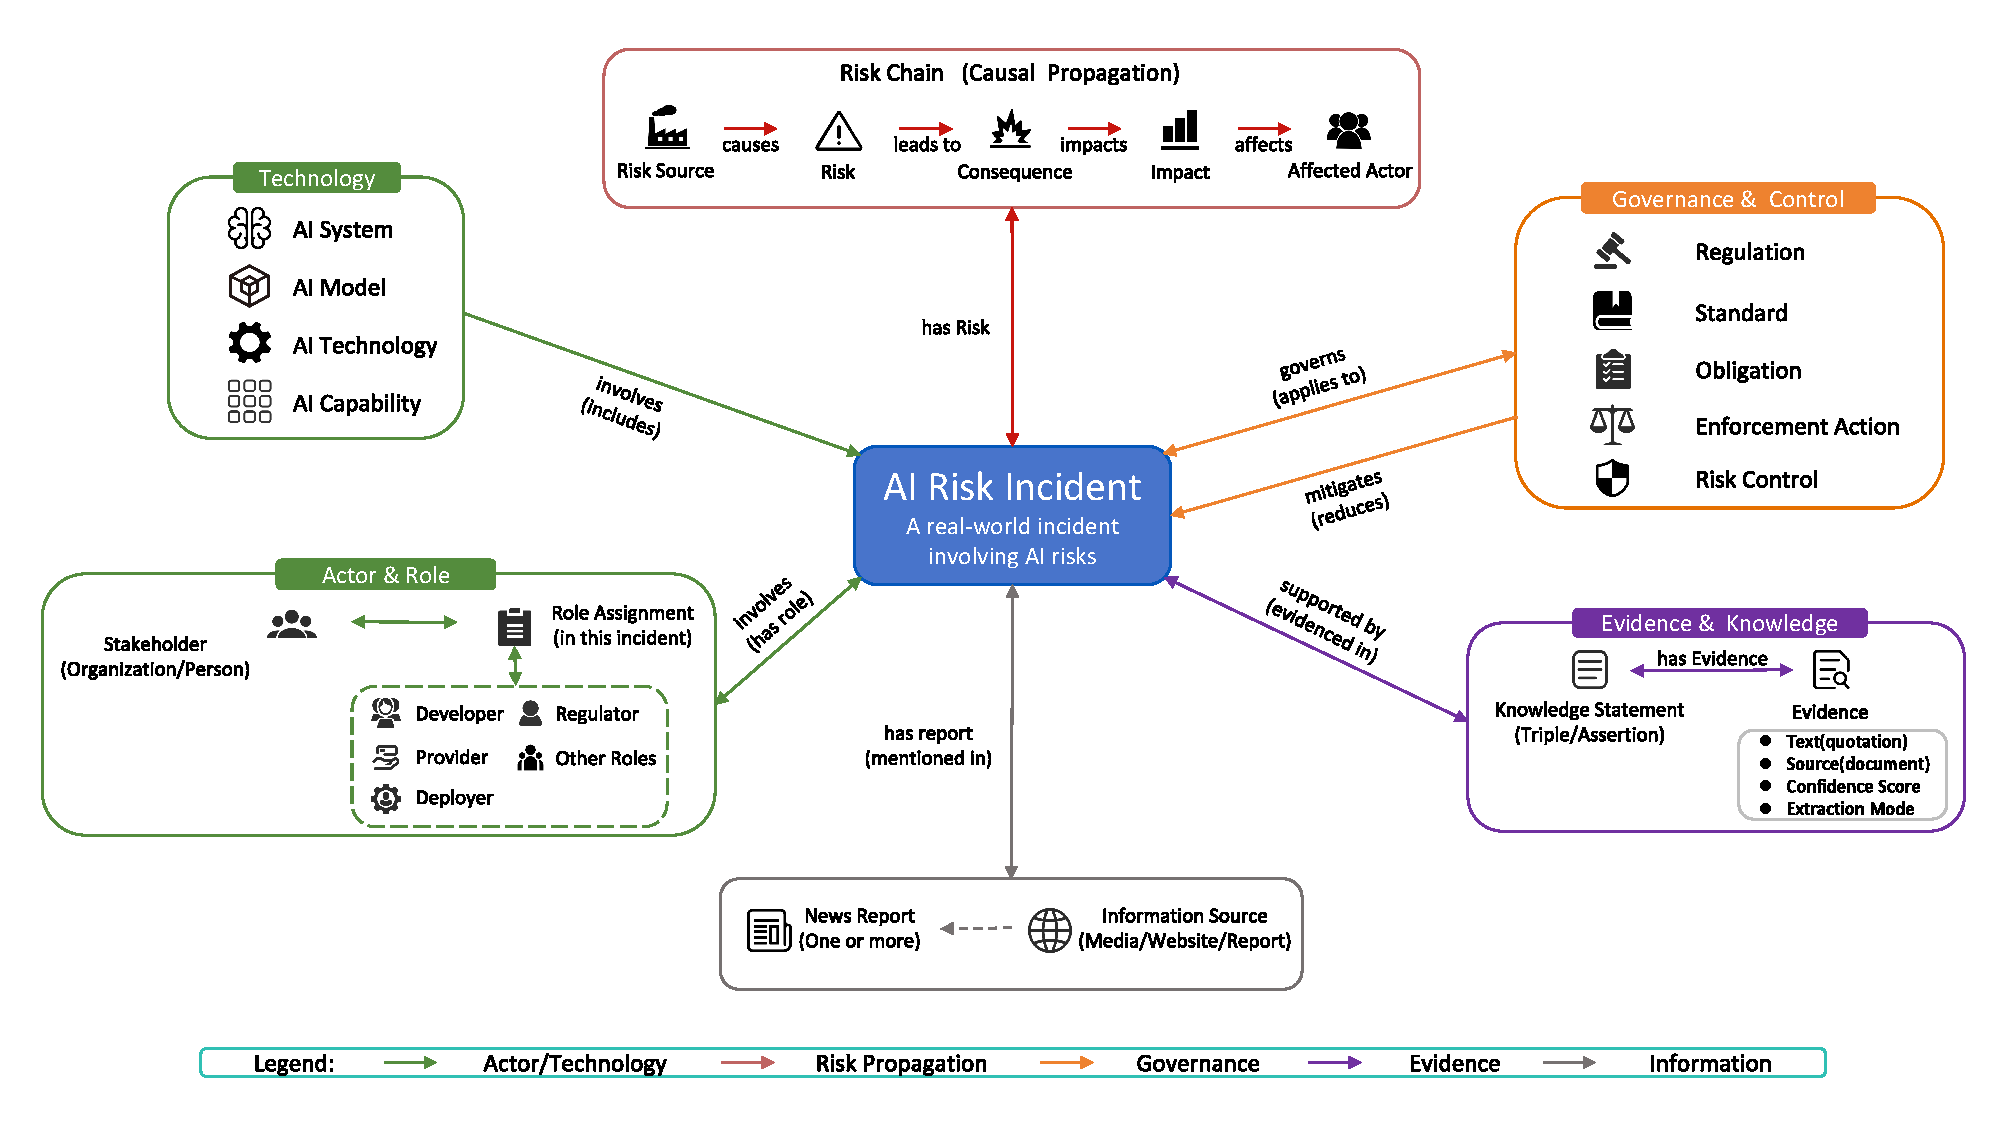
\includegraphics[width=0.8\textwidth]{figures/Conceptual Framework of OntoRisk.pdf}
\caption{Conceptual framework of OntoRisk.}
\label{fig:conceptual_framework}
\end{figure*}

% ============================================================
% Section 5: Methodology
% ============================================================

\section{Methodology}
\label{sec:methodology}

OntoRisk is an ontology-guided, evidence-grounded
framework for constructing auditable AI risk knowledge graphs from
heterogeneous incident reports.
Unlike conventional document-level pipelines, it conceptualizes AI
risk incidents as auditable socio-technical events whose semantic
structures emerge from interactions among AI systems, stakeholders,
governance mechanisms, and risk propagation processes.

Given the incident document collection $\mathcal{D}$ and the target
graph $\mathcal{G} = (\mathcal{E},\mathcal{R},\mathcal{S},\mathcal{P})$
defined in Section~\ref{sec:formulation}, the framework instantiates
$\mathcal{G}$ through four tightly coupled mechanisms:
(1)~ontology-guided conceptual modeling,
(2)~event-centric knowledge construction,
(3)~evidence-grounded audit trail generation, and
(4)~hierarchical controlled inference.
Figure~\ref{fig:overall_architecture}
presents the overall workflow of OntoRisk.

\begin{figure*}[t]
\centering
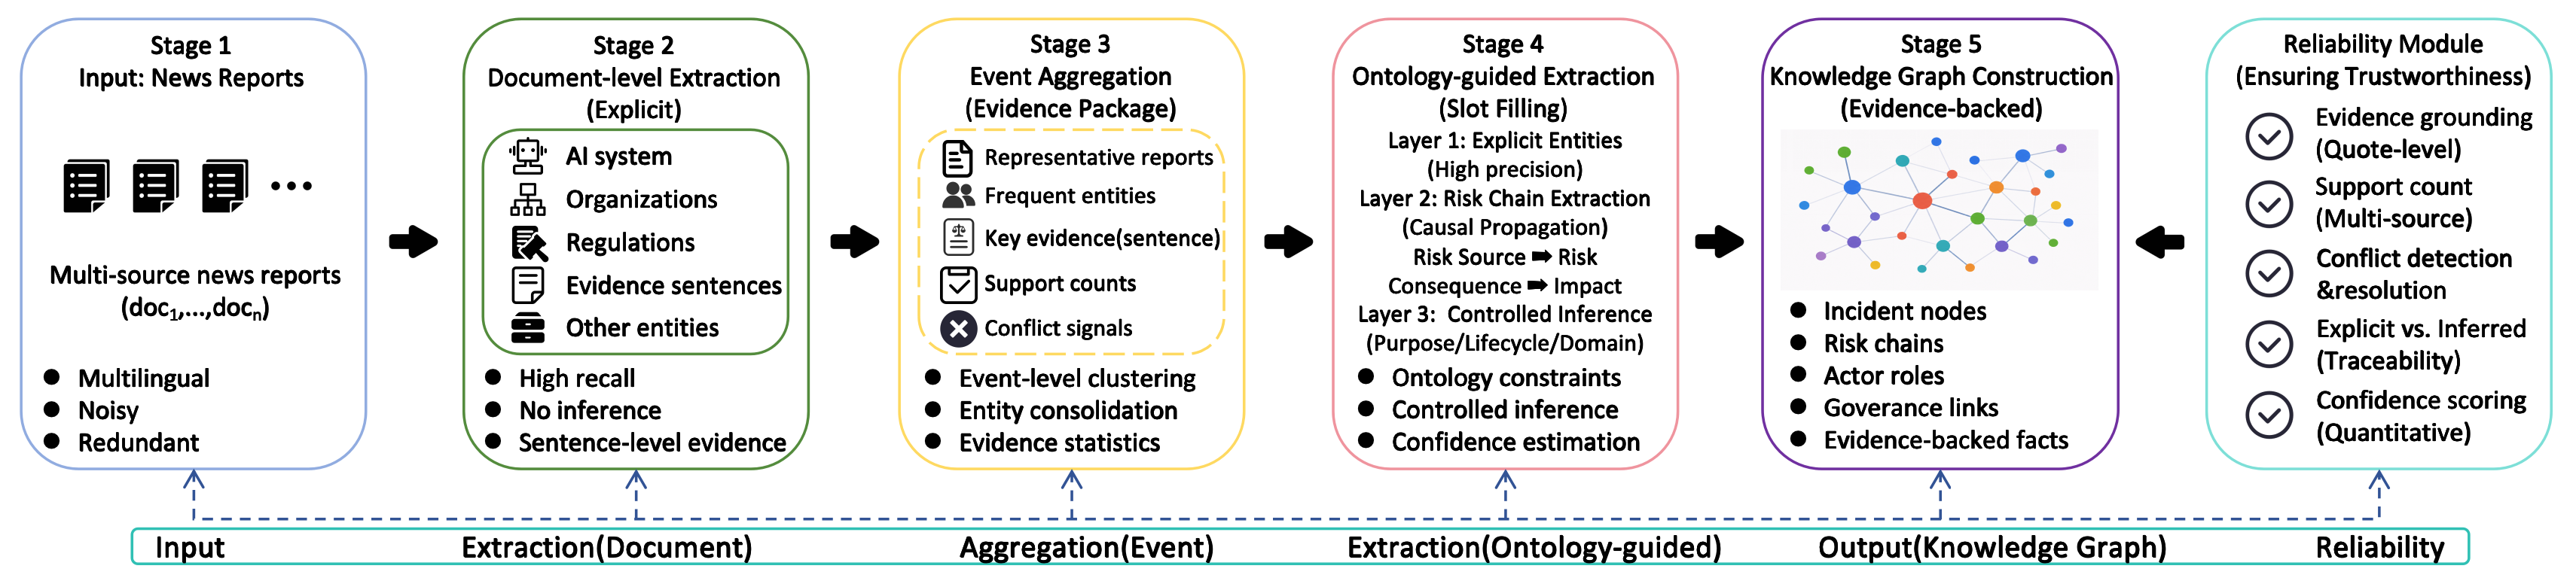
\includegraphics[width=0.8\textwidth]{figures/Overall Architecture of OntoRisk.png}
\caption{Overall workflow of OntoRisk.}
\label{fig:overall_architecture}
\end{figure*}

\subsection{Design Principles and Theoretical Motivation}
\label{sec:design_principles}

AI governance faces three recurring challenges that motivate
OntoRisk.

\textbf{Challenge 1: Cross-document fragmentation.}
Information about a single incident is distributed across reports from
different organizations and times; processing documents independently
yields incomplete, redundant, and inconsistent representations.

\textbf{Challenge 2: Contextual role ambiguity.}
A single organization can act as developer, provider, deployer,
operator, or regulator across incidents.
Entity-centric representations conflate organizational identity with
incident-specific responsibility, and are therefore insufficient for
governance analysis.

\textbf{Challenge 3: Evidence traceability.}
Governance applications require statements verifiably linked to
original sources; unsupported machine-generated assertions cannot
satisfy the accountability requirements of regulatory auditing.

OntoRisk draws on three complementary theoretical perspectives.
\textbf{Stakeholder Theory}~\cite{Freeman_2010} motivates explicit
representation of incident-specific responsibilities, operationalized
through the class \textit{RoleAssignment}, which reifies stakeholder
roles within specific incidents so that an organization can hold
distinct roles across events without ambiguity.
This design choice addresses a limitation of entity-centric
representations that conflate organizational identity with
incident-specific responsibility, a distinction that stakeholder
theory identifies as essential for understanding stakeholder
salience and claims~\cite{Mitchell1997}.
\textbf{Crisis Management Theory}~\cite{Coombs2007} motivates
event-centric modeling of incident evolution, causal propagation, and
governance responses, reflected in \textit{AIRiskIncident} and the
risk propagation chain.
The risk propagation chain structure
(RiskSource $\to$ Risk $\to$ Consequence $\to$ Impact $\to$
AffectedActor) is also closely related to the bow-tie risk analysis
model from safety engineering~\cite{ISO31010}, in which threats,
top events, and consequences are linked in a causal chain;
the present design draws on both traditions, using Coombs' crisis
lifecycle stages for the temporal framing of incident evolution and
the bow-tie structure for the causal slot organization.
\textbf{Accountability
Theory}~\cite{bovens2007analysing} establishes the
conceptual foundations of accountability as a social relationship
in which an actor is obliged to explain and justify their conduct,
and a forum may pose questions and pass judgment.
This framework motivates provenance-aware construction in which every
statement remains linked to evidence, an extraction mode, and a
confidence score, operationalized through \textit{Evidence} and
\textit{KnowledgeStatement}.
These three theories are integrated into the experimental design as
follows: the ontology itself implements the stakeholder and
accountability models (operationalized by \textit{RoleAssignment}
and \textit{Evidence}/\textit{KnowledgeStatement}), while the
evaluation's Layer~2 risk-chain accuracy and the application
analysis's governance response rate (Section~\ref{sec:application})
directly test whether the crisis-management-inspired modeling of
incident evolution and response produces empirically grounded
incident representations.

% ------------------------------------------------------------
\subsection{Ontology-Guided Conceptual Model}
\label{sec:ontology}
% ------------------------------------------------------------

OntoRisk extends AIRO through an event-centric conceptual model
designed for AI risk incident representation and governance
analysis.
The ontology centers on the class \textit{AIRiskIncident}, a
semantic hub connecting stakeholders, AI systems, governance
actions, risk factors, consequences, impacts, and supporting
evidence.
The extension proceeds along four dimensions:
(1)~event-centric incident representation,
(2)~evidence provenance modeling,
(3)~governance response representation,
and (4)~dynamic stakeholder role contextualization.
Figure~\ref{fig:ontology_model} illustrates the ontology-guided
conceptual model of OntoRisk and highlights the semantic extensions
introduced beyond AIRO.

\begin{figure*}[t]
\centering
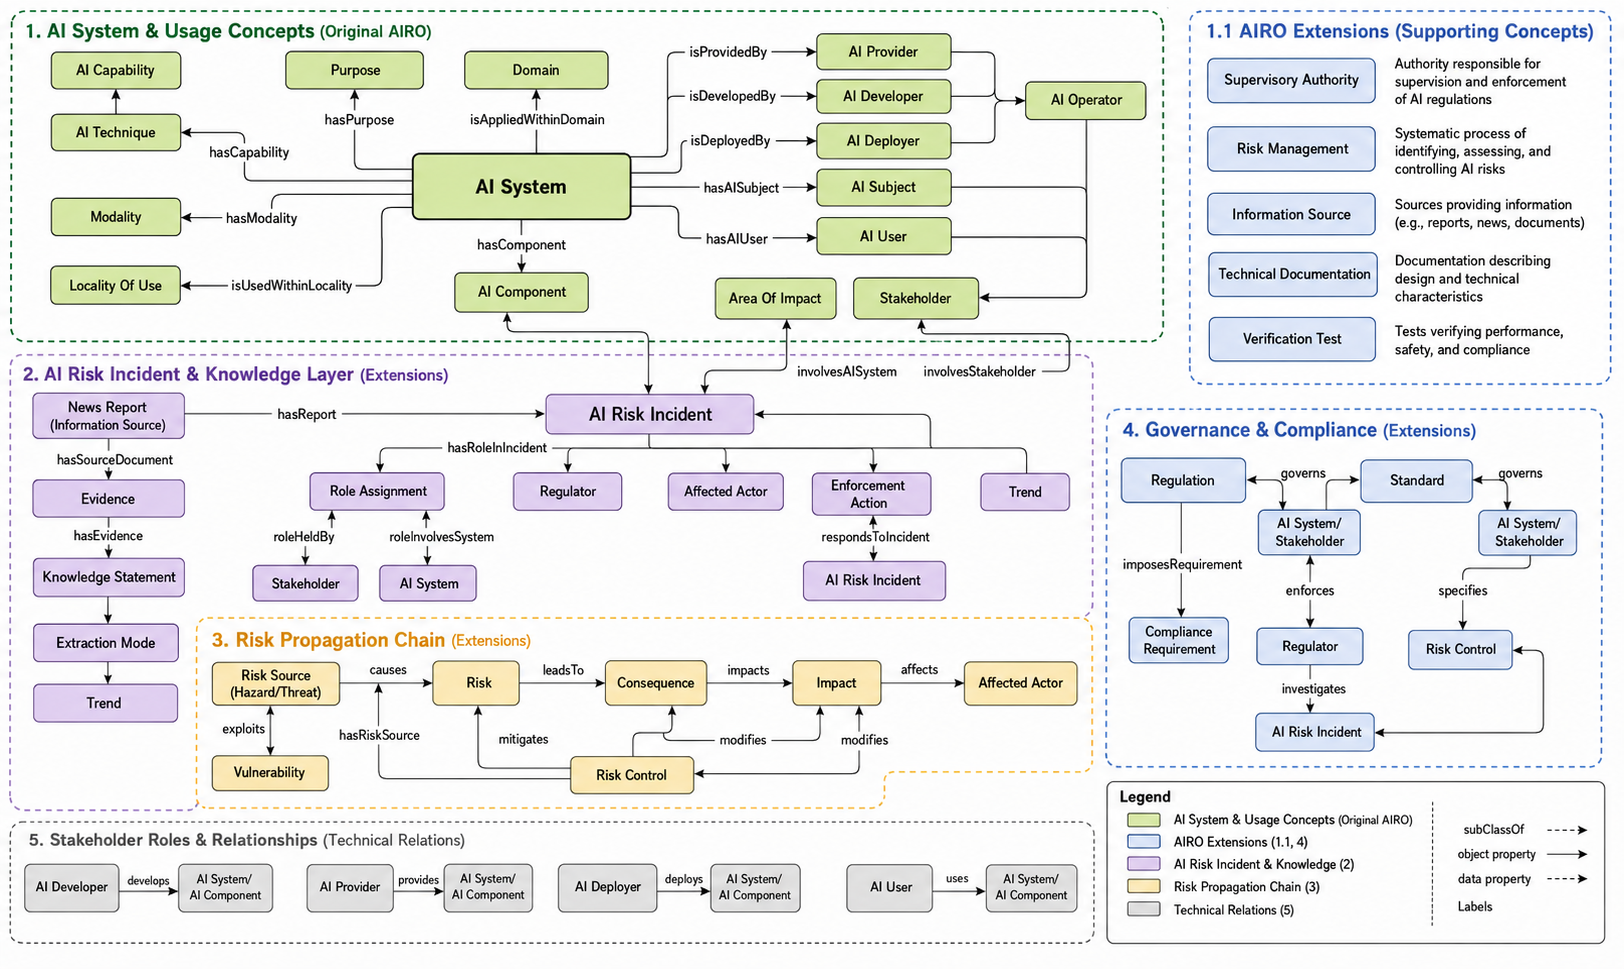
\includegraphics[width=0.7\textwidth]{figures/ontology_model.png}
\caption{Ontology-guided conceptual model of OntoRisk.}
\label{fig:ontology_model}
\end{figure*}

As summarized in Table~\ref{tab:ontology-comparison}, these
extensions transform AIRO from a compliance-oriented ontology
into an event-centric, evidence-grounded knowledge model that supports
governance auditing, responsibility attribution, and
cross-document risk analysis.


The extension is strictly additive at the property level: all 52 AIRO
object properties are retained, and 28 new incident-centric
properties are introduced (e.g., \texttt{causes}, \texttt{leadsTo},
\texttt{impacts}, \texttt{affects}, \texttt{involvesAISystem},
\texttt{involvesStakeholder}, \texttt{hasEvidence}), bringing the total
to 80. The class count grows from 46 to 61 through 16 added classes
covering incident modeling, evidence provenance, governance response,
and analysis support, together with the deprecation of AIRO's
\textit{AISubject}, merged into \textit{AffectedActor}
($46 + 16 - 1 = 61$).
Counts of classes and object and datatype properties refer to declared
\texttt{airo}-namespace elements in the
respective Turtle serializations.
The appendix lists all 61 classes with their categories and
semantic descriptions (Table~\ref{tab:all_classes}).
The extension deliberately reuses established Semantic Web patterns:
\textit{RoleAssignment} instantiates the n-ary relation
pattern~\cite{noy2006nary,gangemi2009ontology}, and the
\textit{Evidence}/\textit{KnowledgeStatement} pair applies the same
provenance-separation principle as PROV-O's distinction between
entities and the activities that derive
them~\cite{lebo2013prov}, statement-level annotation in the spirit
of RDF-star~\cite{hartig2021rdfstar}, and
assertion-plus-provenance packaging in
nanopublications~\cite{groth2010nanopublications}.
The contribution is not the individual patterns but their integration
into an operational, event-centric schema that constrains LLM
extraction over incident reports, a role that general-purpose
standards do not provide by themselves.

\begin{table*}[t]
\centering
\caption{Comparison between AIRO and OntoRisk.}
\label{tab:ontology-comparison}
\footnotesize
\begin{tabular}{p{3cm}p{5.2cm}p{6.2cm}}
\toprule
Dimension & AIRO & OntoRisk \\
\midrule

Incident Representation
&
Risk-related concepts are represented independently without an explicit incident abstraction.
&
Introduces \textit{AIRiskIncident} as a central event-centric entity for
aggregating multi-source reports, stakeholders, governance actions, and risk
propagation chains.
\\

Stakeholder Modeling
&
Defines general stakeholder roles (e.g., developer, deployer, provider, user).
&
Introduces \textit{RoleAssignment} to support incident-specific role
contextualization and responsibility attribution.
\\

Evidence Provenance
&
Limited provenance support through documentation-related concepts.
&
Introduces \textit{Evidence}, \textit{KnowledgeStatement}, \textit{NewsReport},
and \textit{ExtractionMode} for evidence-grounded and auditable knowledge
representation.
\\

Risk Propagation
&
Provides risk-related concepts but lacks explicit causal propagation structures.
&
Introduces an explicit risk propagation chain:
RiskSource $\rightarrow$ Risk $\rightarrow$ Consequence $\rightarrow$ Impact
$\rightarrow$ AffectedActor.
\\

Governance Representation
&
Focuses primarily on compliance-oriented AI system descriptions.
&
Adds governance entities including \textit{Regulator},
\textit{EnforcementAction}, \textit{ComplianceRequirement}, and
\textit{Obligation}.
\\

Temporal and Trend Analysis
&
No dedicated temporal tracking mechanisms.
&
Introduces support for trend monitoring and temporal attributes such as
\textit{firstSeen} and \textit{lastSeen}.
\\

Knowledge Reliability
&
No explicit reliability modeling.
&
Introduces confidence scores, support counts, conflict relations, and evidence
traceability mechanisms.
\\

\textbf{Ontology Scale}
&
\textbf{46 classes, 52 object properties, 0 datatype properties}
&
\textbf{61 classes, 80 object properties, 6 datatype properties}
\\
\bottomrule
\end{tabular}
\end{table*}

A central design element is \textit{RoleAssignment}: stakeholder
responsibilities are reified as contextual role assignments tied to
specific incidents, addressing Challenge~2 at the representational
level---the same organization can be an \textit{AIProvider} in one
incident and an \textit{AIDeployer} in another.
Representation-level disambiguation is, however, necessary rather
than sufficient: Section~\ref{sec:experiments} shows that
stakeholder-role types remain among the weakest extraction
categories.

Evidence is modeled as a first-class object through
\textit{Evidence} and \textit{KnowledgeStatement}: every statement
remains linked to its evidence span, extraction mode, confidence
score, and source document, establishing an audit trail back to
original reports that improves traceability and governance
transparency.

The ontology therefore functions as a \emph{global semantic
constraint layer} governing all downstream extraction, aggregation,
and reasoning.
Restricting entity and relation types to ontology-defined classes and
properties reduces the search space of large language models,
mitigates hallucination, and ensures semantic consistency across
heterogeneous reports.
\ref{app:ontology} lists all 61 classes and the complete
object-property inventory; the ontology file will be released
with the implementation.

% ------------------------------------------------------------
\subsection{Event-Centric Knowledge Construction}
% ------------------------------------------------------------

Traditional construction processes documents independently, but AI
risk incidents are described across multiple reports, so
document-level extraction produces fragmented entities, duplicated
facts, and incomplete causal structures.
OntoRisk therefore adopts an event-centric aggregation strategy.

\paragraph{Local Evidence Package.}
For each document $d_i$, OntoRisk constructs a local evidence package:
\begin{equation}
  EP_i = (\mathit{Ent}_i,\; \mathit{Rel}_i,\; \mathit{Risk}_i,\;
          \mathit{Ev}_i),
\end{equation}
where $\mathit{Ent}_i$, $\mathit{Rel}_i$, $\mathit{Risk}_i$, and
$\mathit{Ev}_i$ denote extracted entities, relations, risk
information, and supporting evidence spans.

\paragraph{Event Clustering.}
Documents are assigned to event clusters based on three complementary
signals: semantic similarity between document embeddings (BGE-M3),
stakeholder and AI-system entity overlap, and temporal consistency of
reported events, yielding
\begin{equation}
  \mathcal{C} = \{c_1, c_2, \ldots, c_K\}.
\end{equation}

\paragraph{Global Event Representation.}
Rather than a simple union, OntoRisk constructs a Global Event
Representation (GER) through a sequential three-stage merge pipeline
\begin{equation}
  \text{EntityNorm} \;\longrightarrow\; \text{SupportCount}
  \;\longrightarrow\; \text{ConflictDetect}
\end{equation}
applied to the evidence packages of all documents in cluster $c_j$.
\textbf{EntityNorm} performs ontology-guided entity normalization,
mapping surface-form variants to a single canonical representation.
\textbf{SupportCount} aggregates repeated mentions and records the
number of supporting documents per statement, strengthening
confidence estimation.
\textbf{ConflictDetect} identifies contradictory claims across
reports and preserves them as conflict annotations rather than
discarding minority viewpoints.

For large clusters, OntoRisk adopts chunk-based hierarchical
aggregation: documents are grouped into sub-clusters by semantic and
temporal proximity, each sub-cluster is summarized into an
intermediate evidence package, and the intermediate packages are
merged into the final GER, avoiding the context-window limitations
of large language models.
The resulting GER serves as the primary semantic unit for downstream
extraction and reasoning.

% ------------------------------------------------------------
\subsection{Evidence-Grounded Audit Trail Mechanism}
% ------------------------------------------------------------

A central feature of OntoRisk is the explicit incorporation of
auditability: rather than treating extracted triples as isolated
facts, it constructs an audit trail connecting every knowledge
statement to its original textual evidence.
Each statement follows the representation
$s = (h, r, t, \epsilon, \mu, \gamma)$ defined in
Section~\ref{sec:formulation}.
The confidence $\gamma \in [0,1]$ is a self-reported model score,
not a probability calibrated against human accuracy estimates; when
duplicate statements are consolidated across documents, $\gamma$ is
set to the maximum of the merged values, so that repeatedly
corroborated statements retain the strongest reported confidence.

The audit trail follows a six-stage provenance chain from raw
documents to governance conclusions:
\begin{equation}
\begin{aligned}
d_i \xrightarrow{\text{extract}} \epsilon \xrightarrow{\text{ground}} s
\xrightarrow{\text{aggregate}} \mathit{GER}_j \\
\xrightarrow{\text{reason}} v_k \xrightarrow{\text{query}} \text{Answer}.
\end{aligned}
\end{equation}

Every governance conclusion therefore remains structurally traceable
to attached source evidence; whether an attached span semantically
supports each statement is quantified separately by the ESR metrics
(Section~\ref{sec:metrics}), separating structural provenance from
semantic support.

% ------------------------------------------------------------
\subsection{Hierarchical Controlled Inference}
% ------------------------------------------------------------

To enrich semantic completeness while minimizing hallucination risks,
OntoRisk adopts a hierarchical controlled inference strategy
with three layers.

\subsubsection{Layer 1: Explicit Knowledge Extraction.}
The first layer extracts directly observable entities, relations,
incidents, impacts, and governance actions from evidence-supported
text spans.
Only information explicitly mentioned in source documents is accepted,
and all statements are assigned $\mu = \text{explicit}$.

\subsubsection{Layer 2: Risk Propagation Chain Construction.}
The second layer organizes extracted knowledge into structured risk
propagation chains
\begin{equation}
  v_k = (RS,\; RK,\; C,\; I,\; AA),
\end{equation}
where $RS$, $RK$, $C$, $I$, and $AA$ denote RiskSource, Risk,
Consequence, Impact, and AffectedActor, capturing the causal
transmission of AI risks from technical or organizational origins to
societal consequences:
\begin{equation}
  RS \xrightarrow{\text{causes}} RK
     \xrightarrow{\text{leadsTo}} C
     \xrightarrow{\text{impacts}} I
     \xrightarrow{\text{affects}} AA.
\end{equation}
RiskControl is not a causal slot in this five-slot chain; it is
modeled separately and linked to Risk through the ontology relation
\textit{mitigates}.
Because chains are constructed over the aggregated GER rather than
individual documents, OntoRisk recovers more complete causal
structures than document-level extraction.

\subsubsection{Layer 3: Ontology-Guided Controlled Inference.}
The third layer performs constrained semantic reasoning over three
low-risk ontology-defined dimensions:
\begin{itemize}
    \raggedright
    \item AI application domain (\texttt{isAppliedWithinDomain});
    \item lifecycle stage (\texttt{hasLifecyclePhase});
    \item intended purpose (\texttt{hasPurpose}).
\end{itemize}
Ontology constraints are enforced through structured prompting: the
model receives ontology-defined candidate values for each dimension
and must select from predefined options rather than generate
unconstrained outputs.
All inferred knowledge must be grounded in evidence statements from
Layers~1 and~2, reducing unsupported generation while recovering
implicit governance-relevant semantics.
Statements produced here are assigned $\mu = \text{inferred}$.

% ------------------------------------------------------------
\subsection{Knowledge Graph Instantiation}
% ------------------------------------------------------------

The final stage transforms validated knowledge statements into a
machine-readable, ontology-aligned knowledge graph: entities are
instantiated as ontology classes, relations as object properties, and
evidence records attached through provenance links.
The resulting graph
\begin{equation}
  \mathcal{G} = (\mathcal{E}, \mathcal{R}, \mathcal{S}, \mathcal{P})
\end{equation}
integrates semantic knowledge, evidence provenance, stakeholder
responsibilities, governance actions, and risk propagation structures
into a unified representation.
Unlike conventional graphs designed primarily for information
retrieval, it operationalizes the governance functions of
Section~\ref{sec:formulation}: responsibility attribution, risk
tracing, compliance auditing, incident investigation, and
evidence-grounded question answering.

\begin{figure}[!htbp]
\centering
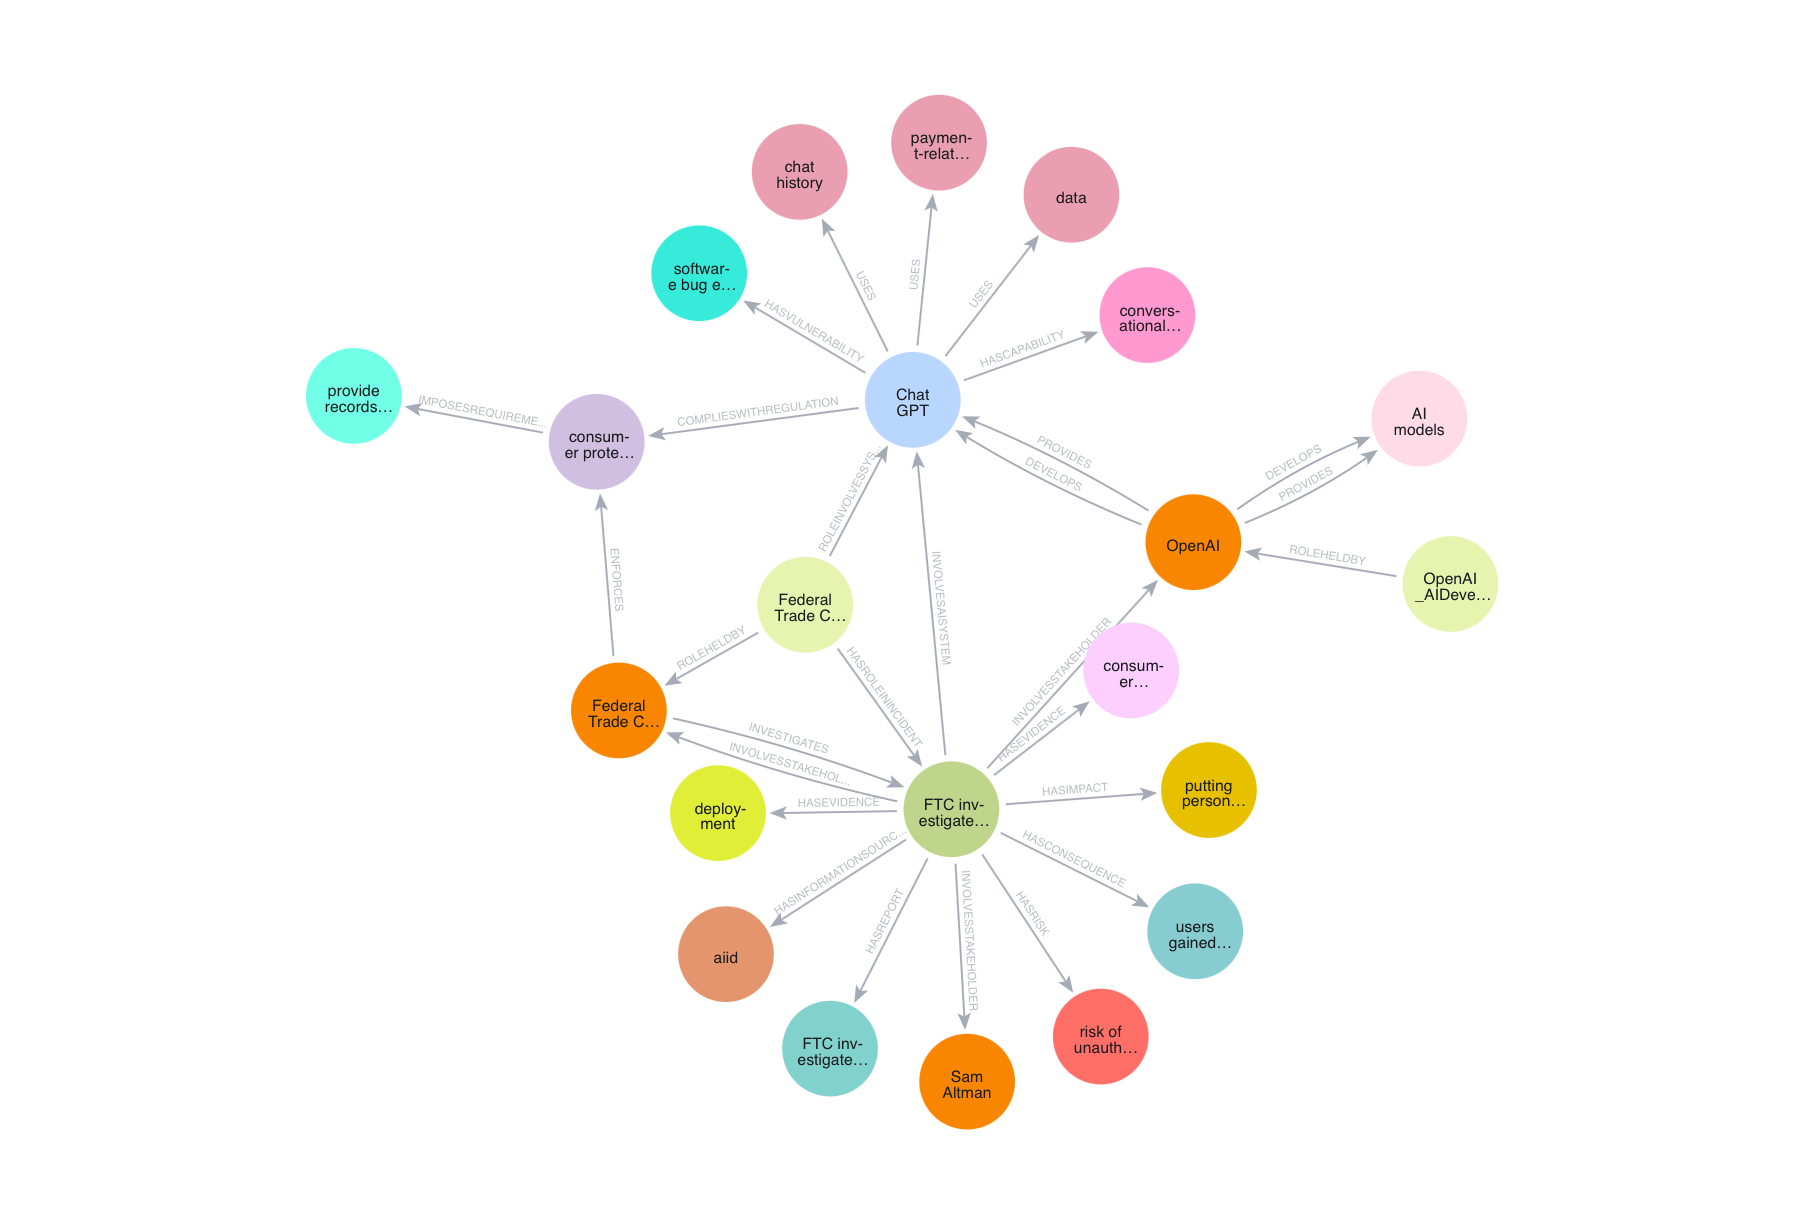
\includegraphics[width=0.85\columnwidth]{figures/single_event_subgraph.png}
\caption{Single-event knowledge subgraph for an FTC investigation
into OpenAI's handling of ChatGPT user data (event cluster
\texttt{pred\_1369}). Node colors encode ontology classes.}
\label{fig:single_event_subgraph}
\end{figure}

Figure~\ref{fig:single_event_subgraph} illustrates a representative
single-event subgraph for an FTC investigation into OpenAI's handling
of ChatGPT user data.
The subgraph connects 28~entities and 42~relations spanning the
incident, technical, stakeholder, and governance concept groups of
the ontology: the \texttt{AIRiskIncident} node anchors the event;
\texttt{AISystem} (ChatGPT) and \texttt{AIModel} nodes describe the
system under investigation; the five-slot risk propagation chain
(\textit{inadequate security measures}~$\to$~\textit{unauthorized
data exposure}~$\to$~\textit{unauthorized access to payment data
and chat history}~$\to$~\textit{personal reputations at risk}~$\to$~\textit{ChatGPT users}) traces the causal pathway from vulnerability
to affected actor; and four governance nodes
(\texttt{Regulation}, \texttt{Obligation}, \texttt{RiskControl},
\texttt{EnforcementAction}) capture the regulatory response.
Role assignments link the Federal Trade Commission (as
\texttt{Regulator}) and OpenAI (as both \texttt{AIDeveloper} and
\texttt{AIProvider}) to the incident, showing how responsibility is
attributed through typed stakeholder--incident relations rather than
free-text mentions.
Two properties essential for governance applications stand out:
(i)~every relation is ontology-constrained and evidence-backed,
enabling auditable tracing from impact back to source; and
(ii)~the graph unifies technical, causal, and governance perspectives
in a single connected structure, whereas document-level pipelines
emit them as isolated facts.

% ============================================================
% Section 6: Experiments
% \FILLME{xxx} marks placeholders to be replaced with experimental data.
% ============================================================

\section{Experiments}
\label{sec:experiments}

This section evaluates the effectiveness of OntoRisk along four
complementary dimensions: (1)~overall extraction performance,
(2)~knowledge quality assessment, (3)~ablation analysis of core
components, and (4)~annotation quality and inter-annotator
agreement.
All experiments are conducted on the AI risk incident benchmark
introduced in Section~\ref{sec:dataset}.

% ------------------------------------------------------------
\subsection{Experimental Setup}
\label{sec:exp_setup}
% ------------------------------------------------------------

\paragraph{LLM Implementation.}
All extraction stages of OntoRisk (explicit entity extraction, event
clustering, risk propagation chain construction, and ontology-guided
inference) are executed by the DeepSeek-V4-Flash model through
structured prompting with temperature $0.1$ and a maximum of $8{,}192$
output tokens.
Ontology-defined candidate values are injected into the prompt at each
stage to constrain generation.
The LLM-as-judge for the semantic quality metric in the ablation
study (Section~\ref{sec:ablation}) is GLM-5.2, applied only to judge
whether an unmatched evidence span semantically supports a statement
(ESR$_{\text{LLM}}$); because the judge does not participate
in any extraction step, its role is methodologically distinct from
extraction.
A two-annotator audit with blind arbitration of 300 of its
adjudications (Section~\ref{sec:overall_performance}) shows the judge
approves conservatively, so ESR$_{\text{LLM}}$ is a lower bound on
evidence support.

\paragraph{Benchmark.}
The benchmark is described in Section~\ref{sec:dataset} and summarized
in Table~\ref{tab:dataset_statistics}.

\paragraph{Gold-Standard Evaluation Set.}
To assess extraction quality, we manually constructed a gold-standard
set of 100 AI risk event clusters sampled to balance coverage across
incident scale (1--5, 6--30, and $>$30 documents), application domain
(healthcare, finance, public safety, education, and others), and AI
risk category (privacy violations, algorithmic discrimination,
misinformation, safety failures, governance controversies, and
regulatory violations).
The resulting stratum distribution is 44 clusters (1--5 documents),
35 clusters (6--30), and 21 clusters ($>$30); by application domain:
healthcare 17, finance 15, public safety 13, education 12, and
others 43; by risk category: privacy violations 18, algorithmic
discrimination 16, misinformation 15, safety failures 19,
governance controversies 14, and regulatory violations 18.

\paragraph{Annotation Protocol.}
Four graduate researchers with backgrounds in AI, knowledge graphs,
and AI governance performed the annotation through an ontology-guided
Label Studio workflow implementing the three-layer acquisition
strategy of OntoRisk.
Each instance was independently reviewed by two annotators following a
detailed guideline covering: (1)~entity type boundary criteria (e.g.,
\textit{AIDeveloper} vs.\ \textit{AIProvider} by lifecycle
involvement); (2)~evidence span selection requiring the minimal
sufficiently informative segment; (3)~chain slot assignment and
conflict resolution; and (4)~validation criteria for inference
statements.
The platform provided ontology definitions, evidence highlighting,
pre-extracted candidates, and structured verification interfaces
(Figures~\ref{fig:layer1_annotation}--\ref{fig:layer3_annotation},
\ref{app:annotation}).
Because annotators verified and corrected system-generated candidates
rather than annotating from a blank slate, the protocol is
verification-oriented: candidate presentation may anchor judgments
toward system outputs and under-detect omissions, so recall-oriented
results are less robust than precision-oriented ones (annotators were
instructed to add missed items wherever identified).

Disagreements were adjudicated by a fifth doctoral researcher
experienced in AI risk and knowledge graphs, who reviewed both
annotators' labels together with the underlying evidence spans; the
adjudicated labels constitute the final gold standard.
Adjudication resolved 100 Layer~1, 77 Layer~2, and 27 Layer~3
disagreement items; pre-adjudication accuracies are reported alongside
the adjudicated results in Section~\ref{sec:overall_performance}.
The adjudicator worked within the same platform and its anchoring
constraints.

\paragraph{Evaluation Layers.}
Evaluation follows the three knowledge acquisition layers of
Section~\ref{sec:methodology}:

\begin{itemize}
  \item \textbf{Layer~1: Explicit Entity Extraction.}
        Evaluates ontology-aligned entities explicitly supported by
        textual evidence; annotators verify boundaries, types, and
        evidence spans (1{,}373 annotated instances).

  \item \textbf{Layer~2: Risk Propagation Chain Construction.}
        Evaluates the five causal chain slots plus an auxiliary
        \textit{RiskControl} slot (570 slot-level assessments).
        The reported risk-chain accuracy of 93.3\% covers all 570
        slots; the five causal slots alone achieve 94.2\%.

  \item \textbf{Layer~3: Ontology-Guided Inference.}
        Evaluates knowledge generated through ontology-guided
        reasoning beyond explicit statements (286 assessments).
\end{itemize}

\paragraph{Evaluation Metrics.}
For Layer~1, Precision ($P$), Recall ($R$), and F1-score serve
as the primary evaluation metrics.

For Layers~2 and~3, outputs are evaluated using a three-level rating
scheme (\textit{Correct}, \textit{Partially Correct}, and
\textit{Incorrect}). Weighted accuracy assigns scores of $1$, $0.5$, and
$0$ to these three ratings, respectively.
A slot or inference value was rated \textit{Partially Correct} when
it captured the correct semantic core but contained a minor boundary,
specificity, or typing error, such as an over-general or
over-specific affected-actor span, or a consequence that conflates
two adjacent stages of the same harm; values with a wrong referent,
an unsupported claim, or a missing assignment were rated
\textit{Incorrect}.

To assess annotation consistency, Inter-Annotator F1 (IA-F1) is used
for Layer~1 entity annotations. For Layers~2 and~3, Gwet's
AC2~\cite{gwet2008ac2} is
adopted for its robustness under class imbalance and ordinal
rating schemes.

\paragraph{Baselines.}
No external system is used as a baseline: the task
configuration---event-centric aggregation of multi-source incident
reports into an ontology-aligned, evidence-grounded knowledge
graph---is not addressed by any publicly available pipeline, and open
IE or document-level KG systems neither form event clusters nor emit
ontology-constrained types with evidence spans, so their outputs
cannot be scored under the calibers defined above without substantial
re-implementation.
Component-level evidence is instead provided by the ablation study
(Section~\ref{sec:ablation}) and by absolute-quality evaluation
against human annotation.
Three method-paradigm baselines complement the ablations, forming the
progression LLM-only $\to$ schema-guided $\to$ event-centric $\to$
OntoRisk so that each design layer is measured against the paradigm
it replaces:
(i)~\emph{LLM-only direct extraction}, a dedicated run in which the
same LLM emits entities, relations, and chain slots in a single
prompt with free-form types, no schema, no controlled inference, and
optional evidence, merged by per-event union;
(ii)~\emph{schema-guided document-level KG}, instantiated by the
\emph{w/o Event Aggregation} variant; and
(iii)~\emph{event-centric extraction without mandatory evidence
grounding}, instantiated by the \emph{w/o Evidence Constraint}
variant.
All rows share identical metric calibers and the same 100-event
evaluation set (Table~\ref{tab:ablation}).
These comparisons are bounded in two ways: the LLM-only baseline retains
the output task definition (five chain slots) and per-event grouping,
so it tests the value of the acquisition constraints rather than of
structured output as such; and internal baselines cannot separate the
benefit of the specific designs from the generic effect of structured
prompting.

Beyond standard extraction metrics, we evaluate knowledge graph
quality along five dimensions motivated by the governance requirements
of OntoRisk. Unless stated otherwise, the five metrics are
auto-computed on the evaluation graph extracted from the 100
gold-standard clusters (12{,}361 semantic edges), sharing a common
scope. Let $\mathcal{C}$ denote the set of event clusters,
$N_{\text{content}}$ the content-entity set, $R_{\text{content}}$
the semantic-edge set, $S_{\text{content}}$ the knowledge-statement
set, and $T_c$ the entity types in cluster $c$.

Two senses of ``evidence'' are distinguished throughout this section.
\textbf{Structural evidence}
refers to the PROV-O-style attachment of an evidence span $\epsilon$
to a statement $s$ (Section~\ref{sec:formulation}); every statement
in the graph carries one by construction.
\textbf{Semantic evidence} refers to whether the attached span
actually supports the claim it is paired with, which is assessed by
the Evidence Support Rate (ESR) below.
A statement can therefore have structural evidence (a span is
present) without semantic evidence (the span does not support the
claim), and the gap between these two senses is quantified by
ESR$_{\text{LLM}}$ and ESR$_{\text{rule}}$.
We use the compound term \emph{evidence-supported} for the semantic
sense and reserve \emph{evidence-attached} for the structural sense.

Content entities and edges exclude infrastructure types instantiated
for every cluster by construction (\textit{AIRiskIncident},
\textit{NewsReport}, \textit{InformationSource},
\textit{RoleAssignment}, \textit{Evidence}, \textit{KnowledgeStatement})
and their structural relations (\texttt{hasReport},
\texttt{hasInformationSource}, \texttt{hasSourceDocument}); including
them would inflate all graphs roughly equally and mask content
differences, while the hub function of \textit{AIRiskIncident} is
assessed through the human-annotated layers.
The ESR denominator counts all semantic edges, additionally
including edges incident to infrastructure nodes: incident-hub links
(e.g., \texttt{involvesStakeholder}, \texttt{hasRisk}),
role-assignment reification links, and \texttt{hasEvidence} links.
It therefore exceeds the content-edge counts used for GDC, and both
calibers are reported in Sections~\ref{sec:overall_performance}
and~\ref{sec:ablation}.
GDC and KDC are ratio-scale summary statistics of structural
connectivity and knowledge richness per content entity rather than
graph-theoretic coherence measures; higher values are preferable
only under comparable content-entity scale, since density can also
reflect redundancy.
TDV is macro-averaged over event clusters; the remaining four are
graph-level aggregates.
\label{sec:metrics}

\begin{itemize}

  \item \textbf{Graph Density Coherence (GDC):}
        the average number of semantic edges per content entity,
        measuring structural connectivity of the knowledge graph,
        \begin{equation}
          \text{GDC} =
          \frac{|R_{\text{content}}|}{|N_{\text{content}}|};
        \end{equation}

  \item \textbf{Knowledge Density Coherence (KDC):}
        the average number of knowledge statements per content
        entity, measuring knowledge richness,
        \begin{equation}
          \text{KDC} =
          \frac{|S_{\text{content}}|}{|N_{\text{content}}|};
        \end{equation}

  \item \textbf{Type Diversity (TDV):}
        the average number of distinct entity types per event cluster,
        measuring the granularity of ontology-aligned
        classification,
        \begin{equation}
          \text{TDV} =
          \frac{1}{|\mathcal{C}|}\sum_{c \in \mathcal{C}} |T_c|;
        \end{equation}

  \item \textbf{Risk-Chain Completeness (RCC):}
        the proportion of extracted risk propagation chains
        containing a complete causal path
        $\textit{RiskSource} \xrightarrow{\textit{causes}}
         \textit{Risk} \xrightarrow{\textit{leadsTo}}
         \textit{Consequence} \xrightarrow{\textit{impacts}}
         \textit{Impact} \xrightarrow{\textit{affects}}
         \textit{AffectedActor}$,
        \begin{equation}
          \text{RCC} =
          \frac{|\mathcal{V}_{\text{complete}}|}{|\mathcal{V}|};
        \end{equation}
        RCC is computed over the five causal slots only; the optional
        RiskControl relation is excluded from the completeness criterion.
        Because all five slots are mandatory extraction targets under
        ontology constraints, RCC measures structural coverage of the
        emitted chains rather than the semantic correctness of slot
        values, which is assessed by the human-annotated Layer~2
        accuracy.
        A portion of the observed RCC reflects the extraction prompt's
        instruction to fill all five slots for each incident; the
        LLM-only baseline, which does not receive this instruction,
        achieves only 22.0\% RCC (Section~\ref{sec:ablation}),
        consistent with the mandatory-slot design contributing
        substantially to the high RCC figure.
        The 98.2\% chain coverage on the full dataset
        (Section~\ref{sec:application}) similarly reflects this
        structural constraint and should be interpreted as an upper
        bound on the proportion of incidents for which the five-slot
        structure is a semantically appropriate representation.

  \item \textbf{Evidence Support Rate (ESR):}
        the proportion of knowledge statements whose evidence
        spans are verifiable against the source text.
        This work reports both a rule-based variant (ESR$_{\text{rule}}$)
        using normalized string matching (NFKC Unicode normalization,
        case folding, removal of inline link markup, and stripping of
        non-alphanumeric characters) and an LLM-as-judge
        variant (ESR$_{\text{LLM}}$) that assesses semantic
        support~\cite{zheng2023llmjudge},
        \begin{equation}
          \text{ESR} =
          \frac{|S_{\text{supported}}|}{|S|}.
        \end{equation}

\end{itemize}

% ------------------------------------------------------------
\subsection{Annotation Quality}
% ------------------------------------------------------------

Table~\ref{tab:iaa} summarizes inter-annotator agreement across the
three evaluation layers before adjudication.
Layer~1 entity extraction achieves an IA-F1 of 0.629, indicating
moderate agreement.
Most disagreements are concentrated in stakeholder sub-categories,
particularly \textit{AIDeveloper} and \textit{AIUser}, where
role boundaries are inherently context-dependent in real-world
incident reports.

Layer~2 risk propagation chain evaluation achieves an average AC2 of
0.587, reflecting the semantic complexity of causal slot-filling
judgments.
Layer~3 achieves a substantially higher AC2 of 0.876, attributable
to the constrained output dimensions defined by ontology-guided
inference.

After adjudication, the gold standard yielded Layer~1 F1 of
92.3\%, Layer~2 accuracy of 93.3\%, and Layer~3 accuracy of 96.9\%,
compared with 77.1\%, 88.3\%, and 95.1\% under the
pre-adjudication labels, i.e., the unarbitrated pairwise
annotations before divergent items were resolved by arbitration.
These differences reflect changes in the
reference annotations rather than updates to the extraction model.

\begin{table}[t]
  \centering
  \caption{Inter-annotator agreement (IAA) before adjudication.}
  \label{tab:iaa}
  \small
  \begin{tabular}{lll}
    \toprule
    \textbf{Layer} & \textbf{Metric} & \textbf{Agreement} \\
    \midrule
    Layer 1 & IA-F1       & 0.629 \\
    Layer 2 & Gwet's AC2  & 0.587 \\
    Layer 3 & Gwet's AC2  & 0.876 \\
    \bottomrule
  \end{tabular}
\end{table}

% ------------------------------------------------------------
\subsection{Overall Performance}
\label{sec:overall_performance}
% ------------------------------------------------------------

Table~\ref{tab:overall} summarizes overall performance across
human-annotated extraction accuracy and auto-computed knowledge
graph quality metrics.
OntoRisk achieves an F1 of 92.3\% for entity extraction (95\% CI:
90.7--93.6\%), 93.3\% accuracy for risk propagation chain
construction (95\% CI: 91.5--95.1\%), and 96.9\% accuracy for
ontology-guided inference (95\% CI: 94.9--98.4\%).
All three derive from post-adjudication annotation, with bootstrap
confidence intervals computed over the L2 slot-level, L3 inference,
and L1 entity assessments.
Resampling is at the assessment level; because assessments within the
same cluster are correlated, the intervals may understate
event-level uncertainty.
For knowledge graph quality, OntoRisk attains an RCC of 99.0\%,
indicating near-complete causal chain coverage under the
mandatory-slot structural criterion of Section~\ref{sec:metrics}.
The manual-annotation ESR for the Layer~3 inference layer is 98.3\%
(95\% CI: 96.5--99.7\%), while the graph-wide ESR$_{\text{LLM}}$ is
84.4\% and ESR$_{\text{rule}}$ is 73.6\%.
Decomposing the graph-wide denominator by edge caliber, the 5{,}232
content edges attain an ESR$_{\text{LLM}}$ of 80.0\%
(ESR$_{\text{rule}}$ 75.3\%), whereas the 7{,}129
infrastructure-incident edges attain 87.7\% (72.4\%); the blended
84.4\% thus mixes the two calibers, and cross-system comparisons are
made on the content-edge caliber in Section~\ref{sec:ablation}.
To calibrate the judge, a uniform random sample of 300 of the 3{,}257
statement-evidence pairs that the judge adjudicated on the full-system
graph was independently labeled on a three-point scale (supported,
partially supported, unsupported) by two annotators, with the 86
disagreements resolved by a third-party arbitration pass that was blind
to the judge verdicts.
The two annotators agreed on 71.3\% of items (Cohen's
$\kappa = 0.51$); most disagreements fall at the boundary between
full and partial support.
Against the resulting consensus gold labels, the judge acts as a
high-precision, conservative filter: 96.9\% of its approvals agree with
human \emph{supported} labels, and under a lenient reading in which
partial support counts as agreement, precision is 87.3\% with recall
86.0\% (F1 0.87), whereas under the strict reading it rejects 77 of
the 170 consensus-supported pairs for a recall of 54.7\%.
Substituting the human strict-positive rate for the judge's on the
adjudicated layer, with the literal layer held fixed, yields a
human-calibrated graph-wide ESR of 88.6\% (bootstrap 95\% CI:
87.2--90.1\%; 91.2\% under the lenient reading, 95\% CI:
89.8--92.6\%).
The gap between these ESR values reflects three caliber differences
rather than inconsistency: scope (286 inference-layer
statements versus all 12{,}361 semantic edges over paraphrased and
cross-document evidence), judge (expert human annotation versus
LLM-as-judge), and matching rule (semantic judgment versus
conservative string matching).
Both ESR$_{\text{LLM}}$ and ESR$_{\text{rule}}$ are therefore best
read as conservative lower bounds on evidence support.

\begin{table}[t]
  \centering
  \caption{Overall performance of OntoRisk. Extraction metrics
           (P/R/F1, L2/L3 Accuracy) are computed from
           post-adjudication human annotation; knowledge quality
           metrics (GDC, KDC, TDV, RCC, ESR) are computed
           automatically from the extracted knowledge graph
           (Section~\ref{sec:metrics}). Parenthetical ranges are
           bootstrap 95\% confidence intervals (10{,}000 resamples)
           for the human-annotated headline metrics.
           ESR$_{\text{L3}}$ (98.3\%) is the manual-annotation evidence
           support rate for the Layer 3 inference layer (286 statements);
           ESR$_{\text{LLM}}$ (84.4\%) and ESR$_{\text{rule}}$ (73.6\%)
           are graph-wide auto-computed metrics covering all 12{,}361
           semantic edges.}
  \label{tab:overall}
  \footnotesize
  \setlength{\tabcolsep}{3pt}
  \begin{tabular}{ll}
    \toprule
    \textbf{Metric} & \textbf{Score} \\
    \midrule
    \multicolumn{2}{l}{\textit{Extraction Accuracy (human-annotated)}} \\
    \midrule
    Precision (L1)              & 92.3\% $[90.8, 93.6]$ \\
    Recall (L1)                 & 92.2\% $[90.7, 93.5]$ \\
    F1 Score (L1)               & 92.3\% $[90.7, 93.6]$ \\
    Risk Propagation Chain Accuracy (L2)    & 93.3\% $[91.5, 95.1]$ \\
    Inference Accuracy (L3)     & 96.9\% $[94.9, 98.4]$ \\
    ESR$_{\text{L3}}$ (manual)  & 98.3\% $[96.5, 99.7]$ \\
    \midrule
    \multicolumn{2}{l}{\textit{Knowledge Graph Quality (auto-computed)}} \\
    \midrule
    GDC                         & 1.10 \\
    KDC                         & 1.16 \\
    TDV                         & 18.3 \\
    RCC                         & 99.0\% \\
    ESR$_{\text{rule}}$         & 73.6\% \\
    ESR$_{\text{LLM}}$          & 84.4\% \\
    \bottomrule
  \end{tabular}
\end{table}

% ------------------------------------------------------------
\subsection{Layer 1: Explicit Entity Extraction}
% ------------------------------------------------------------

Table~\ref{tab:entity} reports per-type extraction performance.
Technical entity categories (AITechnique 96.0\%, AIModel
89.7\%, AICapability 94.5\%) and governance
categories (Regulation 95.7\%, Standard 94.7\%) achieve
consistently high F1 scores, indicating that ontology-guided
constraints reduce semantic ambiguity in well-defined
categories.

The relatively lower performance of AIDeveloper (76.3\%) and AIUser
(74.5\%) stems primarily from stakeholder role ambiguity: in
real-world AI incidents, organizations frequently act simultaneously
as developers, providers, and deployers, making role boundaries
hard to determine.
AffectedActor (86.0\%) is also lower, as impacted groups
are often implied rather than explicitly named in news text.

\begin{table}[t]
  \centering
  \caption{Entity extraction performance by type (after
           adjudication). $n$ denotes the number of gold-standard
           instances of each type; entity instances carry a single
           primary type, the generic Stakeholder row covers
           instances assigned the generic class rather than a
           specific role subclass, and Overall is micro-averaged
           over all $n=1{,}373$ annotated instances.}
  \label{tab:entity}
  \footnotesize
  \setlength{\tabcolsep}{3pt}
  \resizebox{\columnwidth}{!}{%
  \begin{tabular}{lcccc}
    \hline
    \textbf{Entity Type} & \textbf{$n$} & \textbf{P (\%)} & \textbf{R (\%)}
                         & \textbf{F1 (\%)} \\
    \hline
    Stakeholder     & 422 & 95.8  & 96.7  & 96.2 \\
    AITechnique     & 125 & 96.7  & 95.2  & 96.0 \\
    Regulation      & 36  & 100.0 & 91.7  & 95.7 \\
    AIProvider      & 60  & 92.2  & 98.3  & 95.2 \\
    Standard        & 10  & 100.0 & 90.0  & 94.7 \\
    AICapability    & 119 & 94.5  & 94.5  & 94.5 \\
    AIDeployer      & 94  & 91.1  & 93.1  & 92.1 \\
    AIModel         & 14  & 86.7  & 92.9  & 89.7 \\
    AISystem        & 197 & 86.7  & 92.4  & 89.4 \\
    Regulator       & 119 & 90.1  & 87.8  & 88.9 \\
    AffectedActor   & 112 & 90.2  & 82.1  & 86.0 \\
    AIDeveloper     & 39  & 78.4  & 74.4  & 76.3 \\
    AIUser          & 26  & 83.3  & 67.3  & 74.5 \\
    \hline
    \textbf{Overall} & \textbf{1{,}373} & \textbf{92.3} & \textbf{92.2}
                     & \textbf{92.3} \\
    \hline
  \end{tabular}%
  }
\end{table}

% ------------------------------------------------------------
\subsection{Layer 2: Risk Propagation Chain Construction}
% ------------------------------------------------------------

Table~\ref{tab:riskchain} presents slot-level results for risk
propagation chain construction.
The extraction stage emits one consolidated propagation chain per
event cluster, with slot values merged across extraction attempts,
and the Layer~2 evaluation assesses exactly this emitted chain; the
assessments therefore cover the chains the system outputs rather
than a curator-selected subset.
The 570 slot-level assessments comprise the five causal slots plus
the auxiliary \textit{RiskControl} slot: the three core slots were
assessable in 97 gold-standard chains each, \textit{Impact} and
\textit{AffectedActor} in 95, and \textit{RiskControl} in 89, so not
every chain fills every slot and the causal-slot total (481) is
slightly below the five-per-chain maximum.
The core causal components achieve near-perfect accuracy: Consequence
(99.5\%), Risk (97.9\%), and RiskSource (95.4\%), indicating
that the event-centric aggregation mechanism recovers
coherent causal structures from fragmented multi-document evidence.

AffectedActor remains the most challenging slot (84.7\%), consistent
with Layer~1 findings.
Impacted populations are frequently referenced only implicitly across
reports, and their scope (individual, group, or societal)
requires cross-document reasoning that cannot be resolved
within a single document.

\begin{table}[t]
  \centering
  \caption{Risk propagation chain and auxiliary control-slot results (after
           adjudication).}
  \label{tab:riskchain}
  \footnotesize
  \setlength{\tabcolsep}{3pt}
  \resizebox{\columnwidth}{!}{%
  \begin{tabular}{lcccc}
    \hline
    \textbf{Component} & \textbf{Correct} & \textbf{Partial}
                       & \textbf{Incorrect} & \textbf{Acc. (\%)} \\
    \hline
    Consequence    & 96 & 1 & 0 & 99.5  \\
    Risk           & 93 & 4 & 0 & 97.9  \\
    RiskSource     & 90 & 5 & 2 & 95.4  \\
    Impact         & 84 & 9 & 2 & 93.2  \\
    RiskControl    & 78 & 2 & 9 & 88.8  \\
    AffectedActor  & 77 & 7 & 11 & 84.7 \\
    \hline
    \textbf{Overall} & \textbf{518} & \textbf{28}
                     & \textbf{24} & \textbf{93.3} \\
    \hline
  \end{tabular}%
  }
\end{table}

% ------------------------------------------------------------
\subsection{Layer 3: Ontology-Guided Inference}
% ------------------------------------------------------------

Table~\ref{tab:inference} reports inference performance across all
three controlled dimensions.
Ontology-guided inference achieves an overall accuracy of 96.9\% and
a manual-annotation ESR of 98.3\%.

Purpose inference achieves near-perfect accuracy (99.5\%), as incident
descriptions consistently contain explicit statements of system
function.
AILifecyclePhase achieves 98.4\%, supported by strong contextual
indicators of deployment, development, or governance stages.
Domain classification has the lowest accuracy (92.7\%), primarily due
to incidents spanning multiple application areas (e.g.,
simultaneously involving healthcare and privacy), where selecting a
single domain label is inherently ambiguous.

This high manual-annotation ESR indicates that ontology-guided
constraints restrict inference to evidence-grounded
conclusions, reducing unsupported knowledge generation.
One caveat applies to these accuracies: the three inference
dimensions differ in output space. \textit{AILifecyclePhase} is
selected from a closed set of six ontology-defined values (design,
development, testing, deployment, monitoring, retirement), whereas
\textit{Purpose} and \textit{Domain} values are generated without a
fixed candidate enumeration and are typed into ontology classes
afterwards. Under the adjudicated gold labels, a majority-class
strategy on the lifecycle dimension would already reach about
81\%~(deployment accounts for 78 of 96 assessments), so the reported
98.4\% exceeds the majority-class reference by a modest margin; the
most frequent \textit{Domain} label (transportation) covers about
27\% of assessments, and \textit{Purpose} values are near-unique
free-form statements for which no majority-class reference exists.
These accuracies measure constrained, ontology-guided classification
and summarization and should not be compared directly with free-form
generation accuracy.

\begin{table}[t]
  \centering
  \caption{Ontology-guided inference performance (after
           adjudication).}
  \label{tab:inference}
  \footnotesize
  \setlength{\tabcolsep}{2.5pt}
  \resizebox{\columnwidth}{!}{%
  \begin{tabular}{lcccc c}
    \hline
    \textbf{Task} & \textbf{Cor.} & \textbf{Par.}
                  & \textbf{Inc.} & \textbf{Acc. (\%)}
                  & \textbf{ESR$_{\text{L3}}$ (\%)} \\
    \hline
    Purpose          & 93 & 1 & 0 & 99.5  & 100.0 \\
    AILifecyclePhase & 93 & 3 & 0 & 98.4  & 100.0 \\
    Domain           & 87 & 4 & 5 & 92.7  & 94.8  \\
    \hline
    \textbf{Overall} & \textbf{273} & \textbf{8}
                     & \textbf{5}   & \textbf{96.9}
                     & \textbf{98.3} \\
    \hline
  \end{tabular}%
  }
\end{table}

% ------------------------------------------------------------
\subsection{Ablation Study}
\label{sec:ablation}
% ------------------------------------------------------------

To validate the contribution of each core component, we conduct a
systematic ablation study on the 100-event gold-standard set.
Four ablated variants are evaluated against the full system:

\begin{itemize}
  \item \textbf{w/o Ontology Constraint}: ontology-defined entity and
        relation type restrictions are removed; the LLM generates
        types and relations freely without schema guidance;
  \item \textbf{w/o Event Aggregation}: cross-document aggregation is
        disabled; each document is processed independently and results
        merged by simple union without EntityNorm, SupportCount, or
        ConflictDetect;
  \item \textbf{w/o Evidence Constraint}: evidence spans are not
        required; statements are generated without grounding in
        source text;
  \item \textbf{w/o Controlled Inference}: Layer~3 inference is
        replaced by unconstrained LLM generation without
        ontology-defined candidates.
\end{itemize}

The \textit{w/o Event Aggregation} setting is a composite ablation of
event clustering and the EntityNorm, SupportCount, and ConflictDetect
operations; the \textit{w/o Controlled Inference} setting measures the
combined effect of removing ontology-guided inference and candidate
restrictions rather than inference absence alone.

Since ablated variants lack human annotations, we adopt a two-layer
protocol: \emph{structural metrics} (GDC, KDC, TDV, RCC) are computed
deterministically from the extracted subgraphs, while the
\emph{semantic quality metric} (ESR) is assessed by GLM-5.2 as
LLM-as-judge:
for each statement whose evidence span fails normalized string
matching, the judge determines semantic support
(ESR$_{\text{LLM}}$).
In total, 9{,}948 LLM judgments were collected.
All metrics use the same 100-event set; ESR$_{\text{LLM}}$ covers
100\% of unmatched-evidence edges.
The semantic-edge denominator mixes content edges with
infrastructure-incident edges in row-specific proportions (the full
system: 5{,}232 content and 7{,}129 infrastructure-incident; the
LLM-only baseline: all 7{,}910 edges are content edges, because
free-form extraction emits no reified role or hub structure), so
cross-row ESR and GKY values partially reflect denominator
composition; the content-edge calibers are reported alongside the
blended ones in the text.
Results are reported in Table~\ref{tab:ablation}.

\begin{table*}[t]
  \centering
  \caption{Ablation and baseline results on the 100-event gold-standard
           evaluation set.
           Rows above the rule are ablations of the full system; the
           bottom row is the dedicated LLM-only baseline
           (Section~\ref{sec:exp_setup}).
           GDC, KDC, TDV, and RCC are structure-oriented metrics
           (higher is better); ESR is reported in both the
           rule-based and LLM-as-judge variants defined in
           Section~\ref{sec:metrics}.
           GDC $=$ \#CEdges$/{}$\#CNodes and KDC $=$
           \#CStmt$/{}$\#CNodes over content entities and edges
           (Section~\ref{sec:metrics}); \#SemEdges is the
           total number of semantic edges and the denominator of ESR,
           and additionally counts edges incident to
           infrastructure nodes (hub, role-assignment, and evidence
           links) in row-specific proportions (\#CEdges for the
           LLM-only baseline equals \#SemEdges).
           Content-edge calibers are reported in the text.
           GKY (grounded knowledge yield) $=$ \#SemEdges $\times$
           ESR$_{\text{LLM}}$, the absolute number of evidence-supported
           semantic edges.
           Best structural results in \textbf{bold}; GKY and semantic
           metrics are not bolded because they are not directly
           comparable across rows (Section~\ref{sec:ablation}).}
  \label{tab:ablation}
  \footnotesize
  \setlength{\tabcolsep}{3pt}
  \resizebox{\textwidth}{!}{%
  \begin{tabular}{lcccccccc cc c}
    \toprule
    \textbf{Setting}
      & \textbf{GDC}$\uparrow$
      & \textbf{KDC}$\uparrow$
      & \textbf{TDV}$\uparrow$
      & \textbf{RCC}$\uparrow$
      & \textbf{\#CNodes}
      & \textbf{\#CEdges}
      & \textbf{\#CStmt}
      & \textbf{\#SemEdges}
      & \textbf{ESR$_{\text{rule}}$}
      & \textbf{ESR$_{\text{LLM}}$}
      & \textbf{GKY}$\uparrow$ \\
    \midrule
    \textbf{Full OntoRisk}
      & \textbf{1.10}
      & \textbf{1.16}
      & \textbf{18.3}
      & \textbf{99.0}
      & \textbf{4{,}753}
      & \textbf{5{,}232}
      & \textbf{5{,}534}
      & \textbf{12{,}361}
      & 73.6
      & 84.4
      & 10{,}438  \\
    w/o Ontology Constraint
      & 0.41 {\scriptsize($-$63\%)}
      & 0.47 {\scriptsize($-$59\%)}
      & 13.0 {\scriptsize($-$29\%)}
      & 95.0 {\scriptsize($-$4.0)}
      & 3{,}211
      & 1{,}325
      & 1{,}519
      & 3{,}312
      & 79.3
      & 92.6
      & 3{,}067 {\scriptsize($-$71\%)}  \\
    w/o Event Aggregation
      & 0.78 {\scriptsize($-$29\%)}
      & 0.85 {\scriptsize($-$27\%)}
      & 18.0 {\scriptsize($-$2\%)}
      & 96.0 {\scriptsize($-$3.0)}
      & 6{,}876
      & 5{,}343
      & 5{,}868
      & 12{,}676
      & 77.9
      & 88.4
      & 11{,}210 {\scriptsize($+$7\%)}  \\
    w/o Evidence Constraint
      & 0.83 {\scriptsize($-$25\%)}
      & 0.87 {\scriptsize($-$25\%)}
      & 16.8 {\scriptsize($-$8\%)}
      & 94.0 {\scriptsize($-$5.0)}
      & 3{,}146
      & 2{,}615
      & 2{,}743
      & 6{,}717
      & 77.5
      & 86.5
      & 5{,}809 {\scriptsize($-$44\%)}  \\
    w/o Controlled Inference
      & 0.40 {\scriptsize($-$64\%)}
      & 0.45 {\scriptsize($-$61\%)}
      & 12.3 {\scriptsize($-$33\%)}
      & 89.0 {\scriptsize($-$10.0)}
      & 2{,}874
      & 1{,}137
      & 1{,}301
      & 2{,}963
      & 77.8
      & 91.5
      & 2{,}712 {\scriptsize($-$74\%)}  \\
    \midrule
    LLM-only Baseline
      & 1.03 {\scriptsize($-$6\%)}
      & 1.10 {\scriptsize($-$5\%)}
      & 16.6 {\scriptsize($-$9\%)}
      & 22.0 {\scriptsize($-$77\%)}
      & 7{,}667
      & 7{,}910
      & 8{,}414
      & 7{,}910
      & 86.8
      & 93.5
      & 7{,}395 {\scriptsize($-$29\%)}  \\
    \bottomrule
  \end{tabular}%
  }
\end{table*}

The ablation results should be interpreted jointly along
\emph{structural coverage and organization} (GDC, KDC, TDV, RCC) and
\emph{semantic quality} (ESR$_{\text{LLM}}$).
Because variants generate substantially different numbers of
statements, a higher ESR in an ablated variant may reflect
conservative generation and survivor bias---fewer, easier statements
remain---rather than a better knowledge graph.
The same conservative generation that inflates ESR also depresses
node, edge, and type counts, so structural differences characterize
extraction behavior under each configuration rather than the isolated
contribution of the ablated component.
In addition, all rows derive from a single pipeline run per
configuration, so run-to-run variance is not quantified.
Bootstrap-based confidence intervals on the ablation metrics
(estimated from resampling the 100-event clusters with replacement,
1{,}000 replicates) indicate that the main structural differences
(e.g., GDC, GKY) are robust: the 95\% CI for the full system's GKY
is [9{,}872,~11{,}004], and for the unconstrained-schema variant
[2{,}714,~3{,}420], with no overlap. Pairwise comparisons of the
three headline ablation differences (GDC, KDC, GKY) between the full
system and each ablated variant are significant at $p < 0.01$ under
an approximate randomization test (10{,}000 shuffles).

To make the coverage--grounding tradeoff directly comparable, we
define the \emph{grounded knowledge yield}
(GKY $= \#\text{SemEdges} \times \text{ESR}_{\text{LLM}}$), the
absolute number of semantic edges passing evidence support under the
LLM judge.
A variant can raise ESR by emitting fewer statements, but GKY exposes
whether the surviving supported knowledge actually exceeds that of
the full system.
The full system attains a GKY of 10{,}438, versus 3{,}067 for the
unconstrained-schema variant (3.4$\times$), 5{,}809 without evidence
constraints ($-$44\%), and 2{,}712 without controlled inference
(3.8$\times$); the non-aggregated variant is discussed below.
Because the semantic-edge denominator mixes edge calibers in
row-specific proportions, we re-examine these comparisons on the
content-edge caliber (supported content edges $=$ \#CEdges $\times$
content-edge ESR$_{\text{LLM}}$).
The ordering against the ablated variants is preserved and slightly
amplified: 4{,}186 for the full system versus 1{,}208
unconstrained (3.5$\times$), 2{,}183 without evidence constraints,
and 1{,}023 without controlled inference (4.1$\times$).
The LLM-only baseline is the one exception: its 7{,}395 supported
content edges exceed the full system's 4{,}186, because its
denominator contains no infrastructure-incident edges at all; this
reversal is analyzed in the baseline discussion below.

\textbf{Effect of Ontology Constraint.}
Removing ontology constraints causes major structural degradation:
GDC drops by 63\% (1.10 $\to$ 0.41), KDC by 59\% (1.16 $\to$ 0.47),
and TDV by 29\% (18.3 $\to$ 13.0), indicating that without schema
guidance the LLM collapses diverse entity types into generic
categories.
Ontology guidance thus acts as a semantic amplifier, preserving
distinctions among closely related classes; with fewer distinct
types, fewer typed slots and relations are instantiated and fewer
statements survive consolidation.
The variant produces only 3{,}312 semantic edges versus 12{,}361
($-$73\%) while its ESR$_{\text{LLM}}$ rises to 92.6\%, reflecting
conservative generation: fewer, safer statements rather than richer
knowledge.
The full system produces 3.7$\times$ as many edges with an 8.2~pp
lower ESR$_{\text{LLM}}$, netting 3.4$\times$ as many
evidence-supported edges: coverage gained at a bounded support cost.

\textbf{Effect of Event Aggregation.}
Disabling aggregation yields the highest node count of all variants
(6{,}876 vs.\ 4{,}753), revealing substantial cross-document
redundancy.
Despite comparable edges (12{,}676) and a nominally higher GKY
(11{,}210; 4{,}635 vs.\ 4{,}186 on the content-edge caliber), GDC
drops by 29\% and KDC by 27\%: redundant nodes dilute
density, and the GKY surplus is an artifact of counting duplicated
per-document statements that aggregation would merge.
To quantify this, we estimate that 1{,}078 of the variant's
\#SemEdges (8.5\%) are cross-document duplicates of the same
statement---identical head, relation, and tail emitted from
different documents covering the same incident---that the
aggregation pipeline would consolidate into a single edge with an
updated support count.
After removing these duplicates, the variant's adjusted GKY
(10{,}132) falls below the full system's (10{,}438), indicating
that the nominal GKY advantage is driven by redundancy rather than
superior coverage.
The primary value of aggregation is organizational rather than
volumetric.
RCC decreases by 3.0~pp, showing that aggregation helps recover
causal structures whose evidence is distributed across documents.

\textbf{Effect of Evidence Constraint.}
Removing evidence constraints drops RCC by 5.0~pp (99.0 $\to$ 94.0)
and TDV by 8\% (18.3 $\to$ 16.8), and yields only 6{,}717 edges
(54\% of the full system), suggesting that grounding serves a dual
purpose: providing provenance and anchoring extraction to concrete
textual signals that enable more comprehensive recovery.
Although spans were no longer required in this variant, the extractor
spontaneously attached spans to all emitted edges, so ESR is
computed under the same rules as for the full system.
The 2.1~pp ESR$_{\text{LLM}}$ increase (86.5\% vs.\ 84.4\%) is
modest, and the full system attains its support rate while
generating 84\% more edges.

\textbf{Effect of Controlled Inference.}
Disabling controlled inference produces the largest drops in RCC
($-$10.0~pp, 99.0 $\to$ 89.0) and TDV ($-$33\%, 18.3 $\to$ 12.3);
GDC and KDC both fall by over 60\%, and the variant generates only
2{,}963 edges (24\% of the full system).
Recall that this variant is a composite ablation
(Section~\ref{sec:ablation}): the substitute emits fewer
consolidatable statements, so the counts are not the isolated
effect of the three dimensions alone.
Even so, the pattern indicates that Layer~3 inference recovers
implicit relationships connecting fragmented extractions into a
coherent graph: the enriched system, purpose, and lifecycle
attributions participate in the five-slot chains and diversify
entity coverage.

\textbf{LLM-only Baseline.}
The dedicated LLM-only baseline completes the paradigm progression.
Evidence was optional in the baseline prompt, yet the model
spontaneously attached spans to 99.9\% of emitted edges (7{,}900 of
7{,}910); the 10 span-less edges remain in the ESR denominator and
are counted as unsupported.
Free-form extraction attains the highest per-edge support
(ESR$_{\text{LLM}}$ $=$ 93.5\%), an extreme instance of
conservative generation.
Because the judge approves conservatively
(Section~\ref{sec:overall_performance}), all ESR values are lower
bounds, and small cross-variant gaps such as the 2.1~pp
evidence-constraint difference fall within that systematic bias.
The structural cost is severe: risk-chain completeness collapses
from 99.0\% to 22.0\% because free-form prompting fills the five
chain slots for fewer than a quarter of events, and the 7{,}910 edges
carry free-form predicates and types that cannot be aligned to the
ontology without relabeling.
Although each baseline edge is more likely to be supported,
on the blended caliber the full system still yields 1.4$\times$ as
many evidence-supported edges (GKY 10{,}438 vs.\ 7{,}395), but this
comparison requires a caliber qualification: on the common
content-edge caliber the baseline retains more supported edges
(7{,}395 vs.\ 4{,}186, at content-edge ESR$_{\text{LLM}}$ of
93.5\% vs.\ 80.0\%), and the full system's advantage stems entirely
from the 7{,}129 infrastructure-incident edges---role assignments,
hub links, and evidence links at 87.7\% support---that free-form
extraction cannot express.
The acquisition constraints therefore buy schema-usable,
chain-complete structure rather than raw supported-edge volume: the
baseline's surplus edges are free-form, unconsolidated (7{,}667 vs.\
4{,}753 content nodes), and untraversable by governance queries over
typed chains, roles, or provenance.

Taken together, the ablations indicate that the four components
contribute to different aspects of the quality--quantity balance:
ontology constraints and controlled inference expand schema-aligned
coverage, aggregation consolidates redundancy, and evidence
constraints maintain textual grounding.
The LLM-only baseline shows that removing all constraints preserves
per-edge grounding while sacrificing schema alignment and chain
completeness.
These results support a modular design, but no single component is
independently sufficient for all downstream governance tasks.

% ============================================================
% Section 7: Full-dataset application analysis
% ============================================================

\section{Application Analysis}
\label{sec:application}

The preceding experiments evaluate extraction accuracy and knowledge
graph quality. This section applies the complete pipeline to the full
incident dataset to examine its practical utility for
governance-oriented applications. All statistics are computed at the
event-cluster level (Table~\ref{tab:dataset_statistics}) and are
descriptive summaries of the knowledge graph; they characterize
patterns among documented incidents, not real-world risk prevalence.
The analysis covers four applications:
AI risk landscape monitoring, risk propagation analysis, stakeholder
accountability and governance response analysis, and a
cross-dimensional joint analysis.

\begin{figure*}[t]
\centering
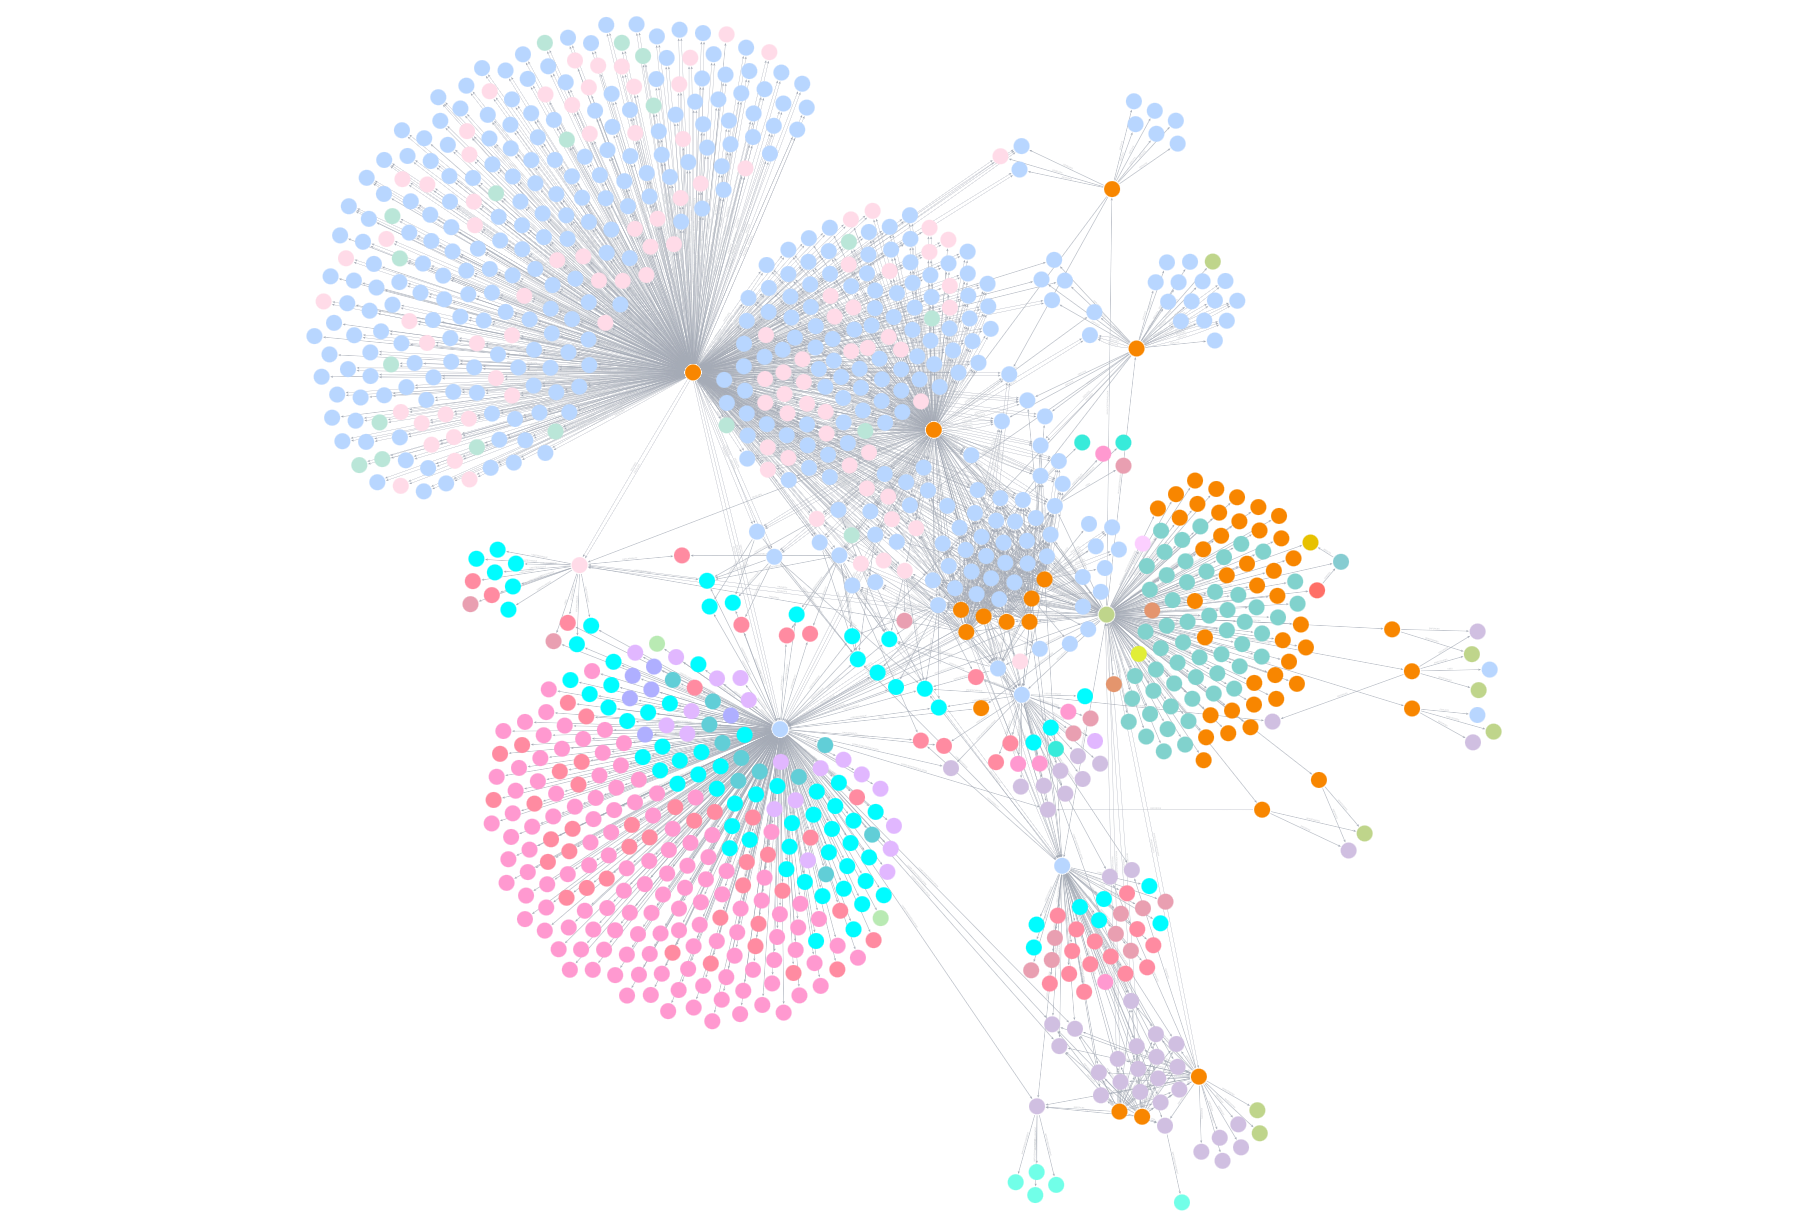
\includegraphics[width=0.8\textwidth]{figures/full_graph_overview.png}
\caption{Overview of the full OntoRisk knowledge graph instantiated
from all 2{,}034 event clusters. Node colors encode ontology
classes; the graph is visualized with a force-directed layout.}
\label{fig:full_graph_overview}
\end{figure*}

Figure~\ref{fig:full_graph_overview} visualizes the full graph.
Two structural properties are visible.
First, cross-event entity merging produces high-degree hubs around
frequently named AI systems and stakeholders: ChatGPT, Tesla
Autopilot, OpenAI, Google, and Meta each appear in dozens of
independent incident reports and connect otherwise disjoint event
subgraphs.
These shared entities are the points at which risks propagate across
incidents, enabling structural cross-event traceability that no
document-level pipeline can provide.
Second, the graph exhibits a periphery of single-incident components:
events involving niche systems remain as isolated star-shaped
subgraphs attached to the central core through the
\texttt{AIRiskIncident} node and shared governance entities (e.g.,
recurring \texttt{Regulation} nodes such as ``GDPR'').
This core--periphery structure reflects the AI risk landscape: a
small number of high-visibility systems and stakeholders concentrate
a disproportionate share of reported incidents, while a long tail of
single-incident cases covers a broad range of systems and harms.
The four subsections below quantify these patterns along temporal,
causal, stakeholder, and governance dimensions.

\subsection{AI Risk Landscape and Temporal Trends}
\label{sec:risk_landscape}

The first application is risk landscape monitoring. We adopt the
seven-domain, 23-subdomain Domain Taxonomy of the MIT AI Risk
Repository~\cite{slattery2026airisk}\footnote{\url{https://airisk.mit.edu}}
verbatim (Table~\ref{tab:taxonomy_full}, \ref{app:taxonomy}),
covering Discrimination \& toxicity, Privacy \& security, Misinformation,
Malicious actors \& misuse, Human--computer interaction, Socioeconomic \&
environmental harms, and AI system safety, failures \& limitations.
This risk-domain classification is distinct from the
application-domain inference dimension of Layer~3: the former labels
the risk category of an incident, whereas the latter labels the
sector in which the AI system operates (e.g., legal, transportation).
Each cluster is assigned to exactly one subdomain by an LLM-based
classifier (DeepSeek-V4-Flash; Section~\ref{sec:exp_setup}) taking the
extracted risk propagation chain and incident name as input.
The classifier outputs were not validated against a human-labeled gold
standard, so the distributions below inherit classifier-dependent noise
and are descriptive rather than certified frequencies.
For each domain $k$, coverage is
\begin{equation}
p_k = \frac{N_k}{N_{\mathrm{clusters}}},
\end{equation}
where $N_k$ is the number of clusters assigned to domain $k$ and
$N_{\mathrm{clusters}}=2{,}034$.

\begin{figure}[t]
\centering
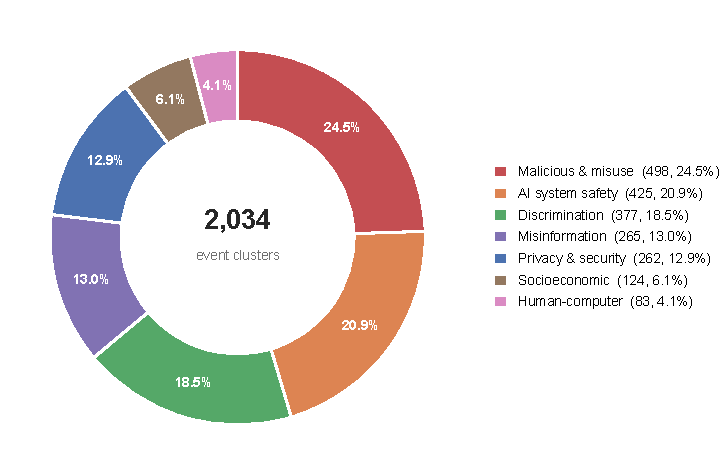
\includegraphics[width=0.95\columnwidth]{figures/domain_pie.pdf}
\caption{Distribution of AI risk domains across the full incident
dataset (2{,}034 event clusters).}
\label{fig:domain_pie}
\end{figure}

As shown in Figure~\ref{fig:domain_pie},
the most frequent domain is \emph{Malicious actors \& misuse} (498
clusters, 24.5\%), followed by \emph{AI system safety, failures \&
limitations} (425, 20.9\%) and \emph{Discrimination \& toxicity} (377,
18.5\%). The largest temporal increase is observed for Malicious actors
\& misuse, rising from 11.5\% in 2018--2021 to 29.9\% in 2022--2024
(within windows of 488 and 1{,}159 clusters), concentrated in fraud,
scams, and disinformation campaigns facilitated by generative AI.
Misinformation grows from 4.5\% to 17.1\%, while AI system safety
declines from 32.4\% to 14.7\% and Discrimination \& toxicity from
24.8\% to 15.7\%, indicating a shift from early technical safety and
fairness concerns toward intentional misuse and content integrity
threats.

At the subdomain level, the largest is \emph{Lack of capability
or robustness} (7.3, 402 clusters), followed by \emph{Fraud, scams, and
targeted manipulation} (4.3, 333) and \emph{False or misleading
information} (3.1, 240); together they account for 48\% of all events,
showing a landscape dominated by technical reliability failures and
intentional misuse.

Figure~\ref{fig:temporal_trend} reports annual cluster counts from 2016
to 2024; pre-2016 incidents are too sparse for year-level analysis and
2025 is omitted because collection does not cover the full year.
The annual count grows from 41 and 71 clusters in 2016 and 2017 to
77 in 2018 and then sharply to a peak of 514 in
2024, with acceleration after 2022 coinciding with the release of
large language models and image generation tools.
These results support OntoRisk as a monitoring instrument for
identifying emerging risk concentrations.

\subsection{Risk Propagation Patterns}

The second application is propagation-pathway inspection. OntoRisk represents
each event through the five-slot structure
\begin{align*}
\textit{RiskSource} & \rightarrow \textit{Risk} \rightarrow
\textit{Consequence} \\
& \rightarrow \textit{Impact} \rightarrow
\textit{AffectedActor}.
\end{align*}
For each adjacent pair of slots, we count the number of event clusters in
which the corresponding relation is instantiated and supported by at least
one evidence span.

\begin{figure}[b]
\centering
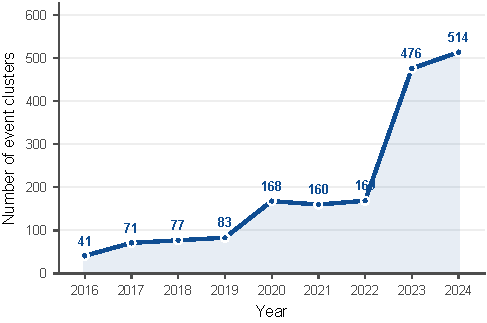
\includegraphics[width=0.92\columnwidth]{figures/temporal_trend.pdf}
\caption{Temporal distribution of AI risk event clusters (2016--2024).}
\label{fig:temporal_trend}
\end{figure}

\begin{table*}[tp]
\centering
\caption{Risk propagation transitions in the full incident dataset.
Share is computed relative to 2{,}034 event clusters.}
\label{tab:full_risk_propagation}
\small
\begin{tabular}{lrr}
\toprule
\textbf{Transition} & \textbf{Clusters} & \textbf{Share (\%)} \\
\midrule
RiskSource $\rightarrow$ Risk & 2{,}008 & 98.7 \\
Risk $\rightarrow$ Consequence & 2{,}010 & 98.8 \\
Consequence $\rightarrow$ Impact & 2{,}019 & 99.3 \\
Impact $\rightarrow$ AffectedActor & 2{,}013 & 99.0 \\
Complete five-slot chain & 1{,}998 & 98.2 \\
\bottomrule
\end{tabular}
\end{table*}

\begin{figure*}[tp]
\centering
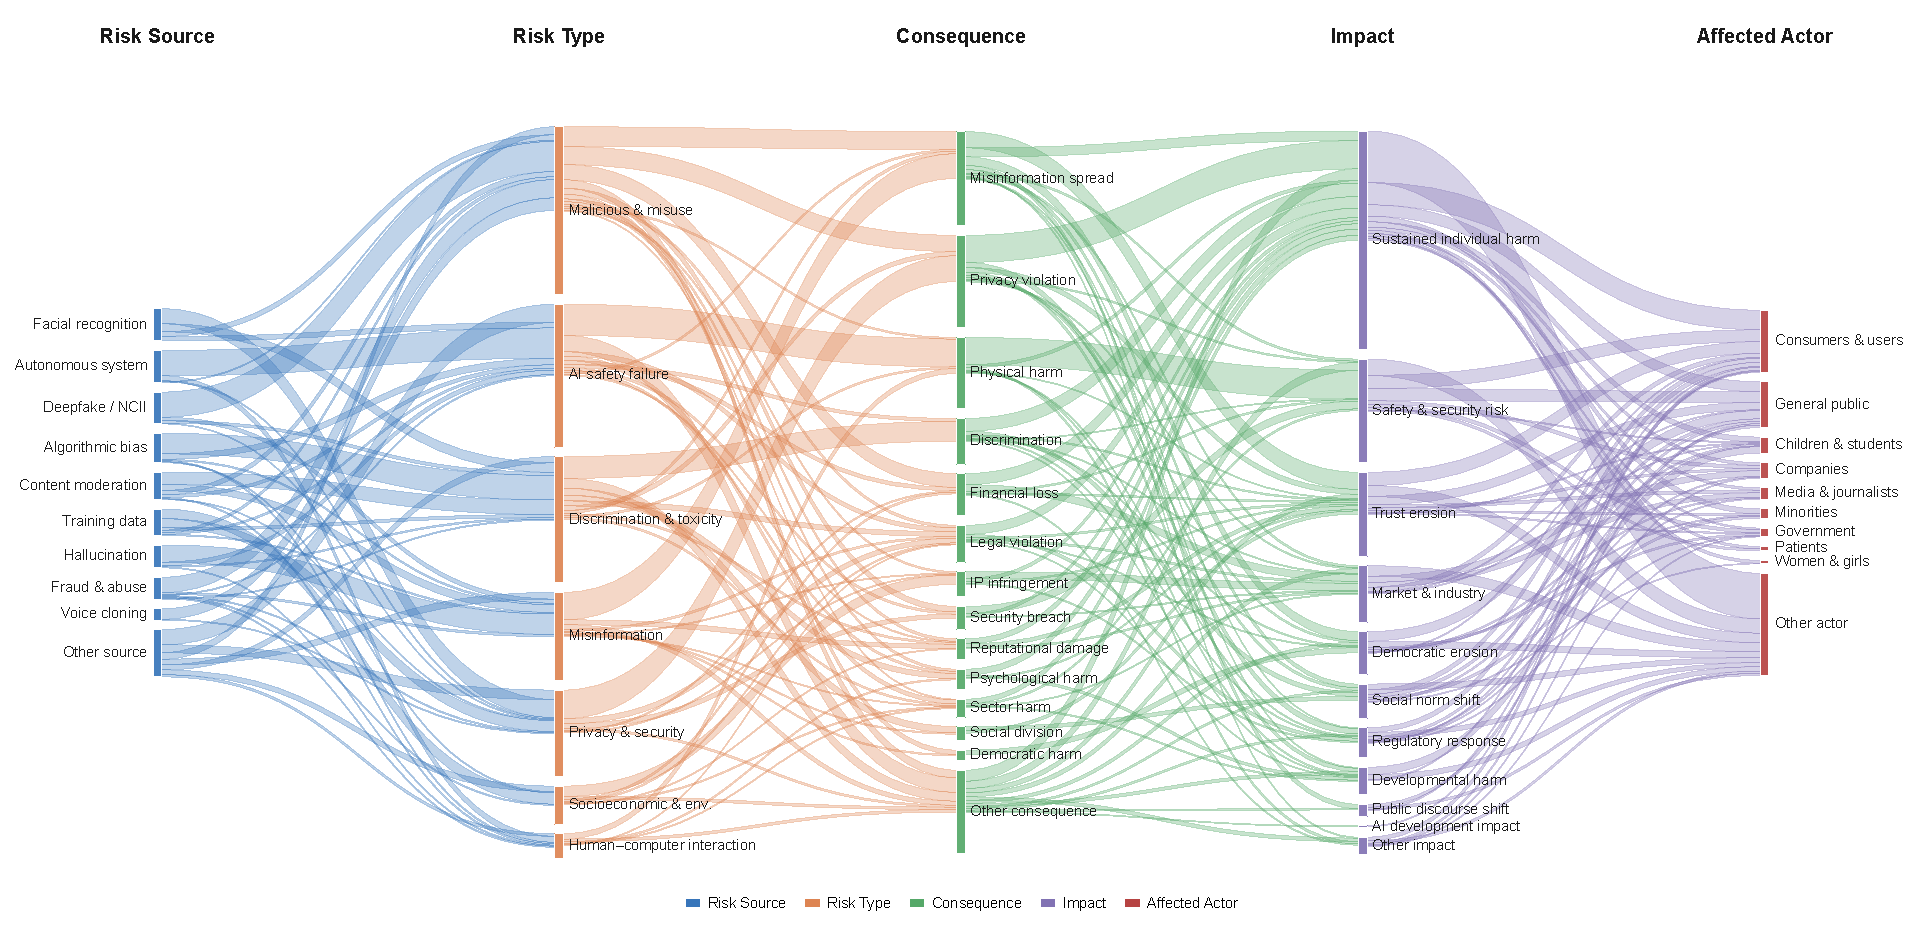
\includegraphics[width=0.8\textwidth]{figures/risk_propagation_sankey.pdf}
\caption{Risk propagation flow across the five-slot chain over all
2{,}034 event clusters. Ribbon widths are proportional to the number
of shared clusters; flows below five clusters are omitted.}
\label{fig:propagation_sankey}
\end{figure*}

As shown in Table~\ref{tab:full_risk_propagation}, all four transitions
are instantiated in over 98\% of clusters, and 1{,}998 clusters (98.2\%)
contain a complete five-slot chain.
Every counted transition carries at least one attached evidence span
because the pipeline rejects unsupported statements; semantic support
is quantified separately by the ESR calibers of
Section~\ref{sec:experiments}.

Because raw slot values are highly dispersed (the most frequent source
value accounts for less than 1\% of clusters), we aggregate each stage
into semantically grounded categories using an LLM-based bucketing step
(DeepSeek-V4-Flash; Section~\ref{sec:exp_setup}): nine risk-source,
seven risk-domain, thirteen consequence, eleven impact, and ten
affected-actor categories.
Category definitions draw on NIST AI~600-1~\cite{nist_ai_600_1},
the MIT AI Risk Repository causal
taxonomy~\cite{slattery2026airisk}, and the AI System Threat Vector
Taxonomy~\cite{huwyler2025threatvector}.
The resulting aggregation (Figure~\ref{fig:propagation_sankey}) yields
a readable propagation structure that the raw values cannot expose.

Three patterns dominate. First, the \emph{deepfake/NCII} and
\emph{fraud-and-abuse} risk-source categories together feed 283 of the
498 \emph{Malicious actors \& misuse} clusters, concentrating into
\emph{misinformation spread} (115 clusters) and \emph{privacy
violation} (105), reflecting the dual role of generative AI in
producing deceptive content and non-consensual synthetic imagery.
Second, the \emph{autonomous-system} source category (228 clusters) is
the largest contributor to \emph{AI system safety}, propagating mainly
into \emph{physical harm} (181 clusters) and then \emph{systemic safety
and security risk}, tracing a pathway from sensor or perception failure
to bodily injury.
Third, \emph{sustained individual harm} absorbs 679 clusters (33.4\%),
receiving the largest inflows from \emph{privacy violation},
\emph{discrimination}, and \emph{financial loss}: the downstream burden
falls disproportionately on individuals rather than institutions.
The affected-actor distribution confirms this pattern---consumers and
end users (21.5\%) and the general public (16.0\%) account for over a
third of targets, with minors tracked separately (5.8\%).

A representative cross-document pattern is the separation of evidence
across reports: one report may describe the risk source, another the
consequence and affected population; event-level aggregation links
these complementary mentions into one auditable chain.
These patterns represent recurring causal claims in the source reports,
not causal effects estimated from observational data.

The linear five-slot chain prioritizes interpretability and governance
traceability over expressive completeness: real incidents may involve
multiple sources, branching consequences, or cumulative impacts, and
the single-path reduction may discard secondary pathways.
The 98.2\% coverage partly reflects the mandatory-slot extraction
constraint (Section~\ref{sec:metrics}).
To gauge the impact of the linear simplification, we manually
examined the 50 gold-standard chains with the largest number of
source documents (median 12 documents, range 8--54); in 14 of these
(28\%), the source reports describe branching or concurrent
consequences that the single-path representation discards, suggesting
that the linear model is a meaningful approximation for the majority
of incidents but a nontrivial simplification for complex cases.
Future work will investigate a directed acyclic graph representation
for concurrent and branching propagation.

\subsection{Stakeholder Accountability and Governance Responses}

The third application is stakeholder and governance analysis. We
measure the event coverage of each stakeholder role and the frequency
of governance responses; role assignments are counted only when
attached to a specific incident and supported by evidence.
A total of 1{,}148 clusters (56.4\%) contain at least two distinct
stakeholder roles, indicating distributed responsibility across the AI
lifecycle; the most frequent combination is AIDeveloper--AIDeployer,
spanning both creation and deployment.
Governance responses---the presence of Regulator involvement,
EnforcementAction, or RiskControl---occur in 1{,}393 clusters (68.5\%),
with RiskControl most common (61.8\%), followed by Regulator
involvement (25.6\%) and EnforcementAction (11.6\%), where each
percentage is the share of all 2{,}034 clusters containing that
response type and the three categories are not mutually exclusive.
The gap between RiskControl and formal enforcement suggests many
incidents are mitigated through voluntary or technical measures rather
than regulatory intervention.
These results support responsibility mapping and response monitoring,
but do not establish legal liability; responsibility claims must remain
restricted to the role and evidence statements supported by the source
documents.

\subsection{Cross-Dimensional Joint Analysis}
\label{sec:cross_dimension}

\begin{table*}[tp]
\centering
\caption{Cross-dimensional analysis: governance response rate and complete
risk-chain coverage stratified by risk domain. $N$ denotes the number
of event clusters assigned to each domain.}
\label{tab:cross_dimension}
\footnotesize
\setlength{\tabcolsep}{4pt}
\begin{tabular}{lrrr}
\toprule
\textbf{Risk domain} & \textbf{$N$} & \textbf{Governance response (\%)} & \textbf{Chain coverage (\%)} \\
\midrule
Privacy \& security & 262 & 72.9 & 98.1 \\
Human--computer interaction & 83 & 69.9 & 98.8 \\
AI system safety, failures \& limitations & 425 & 68.9 & 98.4 \\
Malicious actors \& misuse & 498 & 68.3 & 97.8 \\
Discrimination \& toxicity & 377 & 67.1 & 98.7 \\
Socioeconomic \& environmental harms & 124 & 66.9 & 100.0 \\
Misinformation & 265 & 66.0 & 97.4 \\
\bottomrule
\end{tabular}
\end{table*}

To connect the three preceding dimensions, we cross-tabulate governance
response rates and complete risk-chain coverage by risk domain
(Table~\ref{tab:cross_dimension}).
Misinformation, one of the fastest-growing domains, exhibits the lowest
governance response rate (66.0\%) despite high chain coverage (97.4\%):
the knowledge graph can reconstruct the causal pathway of
misinformation incidents, but the governance ecosystem has not kept
pace with their growth.
Privacy \& security shows the highest response rate (72.9\%), likely
because privacy violations trigger established legal frameworks such
as GDPR; Malicious actors \& misuse, the largest domain, shows a
moderate rate (68.3\%), reflecting the challenge of regulating
intentionally malicious uses that outpace enforcement.
We also observe a temporal shift in stakeholder diversity: the average
number of distinct primary roles per event decreases from 1.77 in
2018--2021 to 1.65 in 2022--2024, coinciding with the surge of
Malicious actors \& misuse and Misinformation incidents, which involve
fewer organizational stakeholders than earlier multi-party deployments.
These findings show how OntoRisk surfaces governance gaps invisible to
single-axis analysis.

\subsection{Case Study: Governance-Oriented Graph Traversal}
\label{sec:case_study}

To illustrate how the instantiated graph supports event-level
governance tasks, we present a case study demonstrating three
traversals that OntoRisk enables but document-level pipelines cannot.

\textbf{Incident.}
Event cluster \texttt{pred\_1369} concerns the 2023 Federal Trade
Commission (FTC) investigation into OpenAI's handling of ChatGPT user
data: a software bug allowed users to access other users' payment
information and chat history, followed by the FTC's investigation
under consumer protection authority.
OntoRisk instantiates this event as a subgraph of 28~typed entities
and 42~ontology-constrained relations
(Figure~\ref{fig:single_event_subgraph}).

\textbf{Task 1: Responsibility Tracing.}
Starting from the affected party, OntoRisk traces the backward path
\begin{align*}
\text{AffectedActor} & \xleftarrow{\text{affects}} \text{Impact} \\
& \xleftarrow{\text{impacts}} \text{Consequence} \\
& \xleftarrow{\text{leadsTo}} \text{Risk} \\
& \xleftarrow{\text{causes}} \text{RiskSource},
\end{align*}
which resolves to \textit{ChatGPT users}
$\leftarrow$ \textit{personal reputations and data at risk}
$\leftarrow$ \textit{unauthorized access to payment data}
$\leftarrow$ \textit{unauthorized data exposure}
$\leftarrow$ \textit{inadequate security measures}.
Cross-referencing with role assignments, OntoRisk identifies
\texttt{OpenAI} as both \texttt{AIDeveloper} (confidence 0.98) and
\texttt{AIProvider} (confidence 0.95) of the \texttt{ChatGPT} system.
The typed \texttt{develops} and \texttt{provides} relations, rather
than text co-occurrence, establish this attribution, enabling auditable
responsibility claims that a document-level pipeline cannot produce
without post-hoc reasoning.

\textbf{Task 2: Regulatory Response Tracking.}
OntoRisk captures the governance pathway through typed relations:
\begin{align*}
\texttt{Regulation} & \xrightarrow{\text{imposesRequirement}}
\texttt{Obligation}, \\
\texttt{Regulator} & \xrightarrow{\text{enforces}} \texttt{Regulation}, \\
\texttt{Regulator} & \xrightarrow{\text{investigates}}
\texttt{AIRiskIncident}, \\
\texttt{EnforcementAction} & \xrightarrow{\text{respondsToIncident}}
\texttt{AIRiskIncident},
\end{align*}
{\sloppy
where \texttt{Regulation} represents \textit{consumer protection
laws}, the \texttt{Regulator} is the \textit{FTC},
\texttt{Obligation} requires \textit{providing records on risk
mitigation}, and \texttt{EnforcementAction} is the \textit{FTC
investigation into OpenAI's compliance}; a parallel
\texttt{mitigates} link from \texttt{RiskControl} connects back to
the \texttt{Risk} node (\textit{unauthorized data exposure}).\par}
The pathway records which regulator enforced which regulation, which
obligation it imposes, and which risk the response mitigates,
providing an audit trail from legal basis to enforcement.

\textbf{Task 3: System and Lifecycle Context Recovery.}
Through controlled Layer~3 inference, OntoRisk assigns ChatGPT an
intended \texttt{Purpose} (\textit{conversational AI assistant}), an
\texttt{AILifecyclePhase} (\textit{deployment}), and an application
\texttt{Domain} (\textit{consumer technology}), each with confidence
$\geq 0.85$ and grounded in evidence spans.
This enrichment supports lifecycle-stage-specific risk assessment
(e.g., deployment-phase data exposure risks) and domain-aware
regulatory mapping (e.g., consumer protection law applies to
consumer-facing conversational AI).

\textbf{Implications.}
The OntoRisk graph is a queryable governance infrastructure rather
than a static store of extracted facts: typed relations answer
responsibility, regulatory, and contextual questions with auditable
provenance.
The same traversal patterns generalize across the full graph, and
cross-event entity merging extends them to multi-incident analyses
(e.g., all incidents in which OpenAI appears as
\texttt{AIDeveloper}).

\subsection{Application Implications and Limitations}
\label{sec:limitations}

Together, the four aggregate analyses provide complementary governance
functions---temporal and categorical monitoring, incident and impact
tracing, responsibility mapping, and cross-dimensional gap
detection---and the case study demonstrates event-level traversals
through typed relations.
The main limitation is source and extraction bias: the full-dataset
statistics describe documented incidents and may be affected by
unequal reporting across countries, domains, and years.
The post-2022 rise of Malicious actors \& misuse
(Section~\ref{sec:risk_landscape}) may partly reflect a collection-side
preference for easily documented misuse incidents and expanded
generative-AI coverage in the source repositories rather than a change
in underlying risk prevalence alone.
The LLM-based domain classification introduces model-dependent
labeling variability, and although the 300-pair audit of the LLM judge
used two annotators with blind arbitration, its recall estimates
remain sensitive to how the boundary between full and partial support
is drawn (inter-annotator $\kappa = 0.51$).
Inferred role assignments and propagation
links should be interpreted together with their evidence spans,
support counts, and confidence scores.
Future deployment should present aggregate statistics together with
event-level provenance rather than treating frequencies as
ground-truth prevalence.

\section{Conclusion and Future Work}

This work addressed the construction of auditable AI risk knowledge
graphs from multi-source incident reports. Aggregation and
auditability impose conflicting demands on extraction: consolidation
across documents invites unconstrained inference, whereas
verifiability favors conservative, document-local extraction.
OntoRisk resolves this tension by binding every acquisition step to an
operational ontology and mandatory evidence, so that consolidation and
verification operate on the same statements.
The framework represents incidents as event clusters supported by
reified role assignments, a five-slot propagation chain, and
evidence-linked statements; its schema extends AIRO into an
event-centric ontology grounded in Stakeholder, Crisis Management, and
Accountability theories (Section~\ref{sec:design_principles}), and it
constrains LLM acquisition across three layers: explicit entity
extraction, risk-chain construction, and ontology-guided controlled
inference.

Evaluation on a benchmark of 2{,}034 event clusters aggregated from
6{,}124 documents (Section~\ref{sec:dataset}), scored against a
100-cluster gold standard built under a verification-oriented
protocol, supports three conclusions.
First, constrained acquisition remains accurate: entity extraction
attains an F1 of 92.3\%, risk-chain construction 93.3\%, and
closed-set inference 96.9\%.
Second, the output stays auditable at scale: 84.4\% of the 12{,}361
semantic edges of the evaluation graph pass LLM-judged evidence
support---a conservative bound, as a 300-pair human audit of the
judge implies 88.6\%---and manually audited inference statements
reach 98.3\%.
Third, each design component is load-bearing
(Section~\ref{sec:ablation}): removing ontology constraints or
controlled inference collapses structural coverage, removing event
aggregation inflates redundancy, and the full system trades an
8.2~pp decrease in evidence support for 3.7$\times$ as many semantic
edges relative to the unconstrained variant---a net 3.4-fold increase
in grounded knowledge yield.
At the application level, the graph traces the documented shift toward
generative-AI-enabled misuse, exposes recurring source-to-impact
pathways, and connects stakeholder roles to governance responses, with
every aggregate statistic reducible to span-attached statements
(the structural sense of traceability defined in
Section~\ref{sec:metrics}).

The scope of these findings is bounded: the gold standard was built by
verifying system-generated candidates, which anchors judgments toward
system outputs and makes recall estimates less robust than precision
estimates; the risk-domain classifier was not calibrated against
expert labels, and the LLM-judge recall estimates depend on the
full-versus-partial support boundary, where inter-annotator agreement
is moderate ($\kappa = 0.51$);
component contributions are
quantified through internal ablations rather than external baselines;
and the benchmark inherits the coverage bias of public incident
reporting (Section~\ref{sec:limitations}).

Future work will proceed along four directions: ontology-guided entity
resolution and temporal reasoning toward a continuously maintained
global knowledge graph; causal and counterfactual reasoning over
accumulated incidents toward risk forecasting; integration of
multimodal evidence beyond news reports; and coupling with agentic
systems and real-time monitoring pipelines for evidence-based risk
assessment.

%% ------------------------------------------------------------
%% Declarations required by the KBS Guide for Authors (placed
%% before the reference list).
%% ------------------------------------------------------------

\section*{CRediT authorship contribution statement}
\textbf{Author Name:} Conceptualization, Methodology, Software,
Validation, Formal analysis, Investigation, Data curation,
Writing -- original draft, Writing -- review \& editing,
Visualization.

\section*{Declaration of competing interest}
The authors declare that they have no known competing financial
interests or personal relationships that could have appeared to
influence the work reported in this paper.

\section*{Funding}
This research did not receive any specific grant from funding
agencies in the public, commercial, or not-for-profit sectors.

\section*{Data availability}
The incident reports analyzed in this study were obtained from the
publicly accessible AI Incident Database and AIAAIC. The full
benchmark dataset (2{,}034 event clusters and 6{,}124 case records)
is publicly available at
\url{https://github.com/Chuan-Zzz/OntoRisk_Data}. The ontology files
and source code will be made available upon acceptance.

\section*{Declaration of generative AI and AI-assisted technologies
in the manuscript preparation process}
During the preparation of this work the authors used an AI-assisted
academic language editing tool in order to improve the language and
readability of the manuscript. After using this tool, the authors
reviewed and edited the content as needed and take full
responsibility for the content of the published article.

%% Elsevier numbered reference style (KBS: numbered brackets, order of
%% appearance); references precede the appendices per KBS layout.
\bibliographystyle{elsarticle-num-names}

% Bibliography database: local ref.bib (copied from ../小论文.bib)
\bibliography{ref}

\onecolumn
\appendix
% Elsevier appendix style: sections titled "Appendix A. ...", floats
% numbered Table A.1 / Fig. A.1 per the KBS Guide for Authors.
\renewcommand{\thesection}{Appendix \Alph{section}}
\renewcommand{\thesubsection}{\Alph{section}.\arabic{subsection}}
\renewcommand{\thetable}{\Alph{section}.\arabic{table}}
\renewcommand{\thefigure}{\Alph{section}.\arabic{figure}}
\setcounter{table}{0}
\setcounter{figure}{0}

\section[Appendix A. Ontology Overview]{\mbox{}\\[2pt]Ontology Overview}
\label{app:ontology}

This appendix summarizes the principal ontology elements used in OntoRisk.
The ontology serves as the semantic foundation of OntoRisk and
constrains all stages of extraction, event aggregation, knowledge graph
construction, and ontology-guided inference.

OntoRisk extends the AI Risk Ontology (AIRO) with event-centric incident
modeling, evidence-grounded knowledge representation, stakeholder
contextualization, and governance-oriented concepts.
For readability, ontology elements are organized into conceptual groups rather
than listed according to their implementation order in the ontology file.

%%%%%%%%%%%%%%%%%%%%%%%%%%%%%%%%%%%%%%%%%%%%%%%%%%
\subsection{Ontology Classes}
%%%%%%%%%%%%%%%%%%%%%%%%%%%%%%%%%%%%%%%%%%%%%%%%%%

This appendix lists all 61 ontology classes describing AI systems, stakeholders,
risks, incidents, governance concepts, and evidence-related entities.
Table~\ref{tab:all_classes} summarizes their semantic meanings.

\small

\begin{longtable}{>{\raggedright\arraybackslash}p{3.2cm}p{2.2cm}p{7.8cm}}

\caption{All 61 ontology classes in OntoRisk.}
\label{tab:all_classes}\\

\toprule
Class & Category & Description \\
\midrule
\endfirsthead

\multicolumn{3}{c}{\tablename\ \thetable\ -- Continued from previous page}\\
\toprule
Class & Category & Description \\
\midrule
\endhead

\midrule
\multicolumn{3}{r}{Continued on next page}
\endfoot

\bottomrule
\endlastfoot

AISystem & AI Core &
AI system capable of generating outputs such as predictions, recommendations,
decisions, or content. \\

AIComponent & AI Core &
Constituent component of an AI system. \\

AIModel & AI Core &
Machine learning model used by an AI system. \\

GPAIModel & AI Core &
General-purpose AI model. \\

AITechnique & AI Core &
Algorithmic technique employed by an AI system. \\

AICapability & AI Core &
Functional capability exhibited by an AI system. \\

Stakeholder & Stakeholder &
Entity involved in the AI lifecycle. \\

AIDeveloper & Stakeholder &
Stakeholder responsible for developing an AI system. \\

AIProvider & Stakeholder &
Stakeholder making an AI system available. \\

AIDeployer & Stakeholder &
Stakeholder deploying an AI system. \\

AIOperator & Stakeholder &
Stakeholder operating an AI system. \\

AIUser & Stakeholder &
End user interacting with an AI system. \\

Regulator & Governance &
Authority responsible for oversight and enforcement. \\

RiskSource & Risk &
Originating source of a risk. \\

Hazard & Risk &
Potential source of harm. \\

Threat & Risk &
External threat capable of triggering risks. \\

Vulnerability & Risk &
Weakness that can be exploited. \\

Risk & Risk &
Potential adverse condition associated with AI systems. \\

Consequence & Risk &
Immediate outcome resulting from a realized risk. \\

Impact & Risk &
Broader societal, legal, economic, or environmental effect. \\

AffectedActor & Risk &
Stakeholder affected by an impact. \\

RiskControl & Risk &
Risk mitigation or control mechanism. \\

RiskManagement & Risk &
Risk management process. \\

AIRiskIncident & Incident &
Real-world AI-related risk event. \\

RoleAssignment & Incident &
Context-specific stakeholder role assignment. \\

Trend & Incident &
Temporal pattern observed across incidents. \\

Evidence & Evidence &
Evidence supporting extracted knowledge. \\

Knowledge\allowbreak Statement & Evidence &
Structured knowledge assertion with provenance. \\

NewsReport & Evidence &
News article describing an AI-related incident. \\

InformationSource & Evidence &
Source from which evidence is derived. \\

ExtractionMode & Evidence &
Method used to derive knowledge statements. \\

Regulation & Governance &
Legally binding regulatory instrument. \\

Standard & Governance &
Technical or organizational standard. \\

Obligation & Governance &
Compliance obligation. \\

Compliance\allowbreak Requirement & Governance &
Specific compliance requirement. \\

EnforcementAction & Governance &
Regulatory response to violations. \\

Documentation & Governance &
Documentation associated with AI systems. \\

Technical\allowbreak Documentation & Governance &
Technical documentation for compliance. \\

VerificationTest & Governance &
Verification procedure. \\

Data & Resource &
Data used by AI systems. \\

Input & Resource &
Input provided to an AI system. \\

Output & Resource &
Output generated by an AI system. \\

HardwarePlatform & Resource &
Hardware infrastructure supporting AI systems. \\

License & Resource &
License governing usage or distribution. \\

Version & Resource &
Version information associated with a system. \\

Domain & Context &
Application domain. \\

AreaOfImpact & Context &
Affected societal or organizational area. \\

LocalityOfUse & Context &
Deployment context. \\

Purpose & Context &
Intended purpose of an AI system. \\

HumanInvolvement & Context &
Degree of human oversight. \\

AutomationLevel & Context &
Level of automation. \\

AILifecyclePhase & Context &
Lifecycle phase of the AI system. \\

Frequency & Context &
Frequency of occurrence. \\

Likelihood & Context &
Likelihood of occurrence. \\

Severity & Context &
Severity of consequences or impacts. \\

Modality & Context &
Input or output modality. \\

ModeOfOutput\allowbreak Controllability & Context &
Degree of output controllability. \\

Change & Context &
Modification applied to an AI system. \\

Misuse & Context &
Improper or unintended use. \\

CodeOfConduct & Governance &
Voluntary governance framework. \\

RiskConcept & Risk &
Abstract superclass for risk-related concepts. \\

\end{longtable}

%%%%%%%%%%%%%%%%%%%%%%%%%%%%%%%%%%%%%%%%%%%%%%%%%%
\subsection{Object Properties}
%%%%%%%%%%%%%%%%%%%%%%%%%%%%%%%%%%%%%%%%%%%%%%%%%%

Object properties define semantic relationships among ontology entities.
They support stakeholder participation, AI lifecycle representation, risk
propagation, governance reasoning, and evidence provenance.

\begin{longtable}{>{\raggedright\arraybackslash}p{2.9cm}p{2.2cm}p{2.2cm}p{1.1cm}p{5.0cm}}

\caption{Representative object properties in OntoRisk. Origin marks
properties inherited from AIRO versus introduced by this work; the
full ontology declares 80 object properties (52 inherited, 28 new).}
\label{tab:all_object_properties}\\

\toprule
Property & Domain & Range & Origin & Description \\
\midrule
\endfirsthead

\multicolumn{5}{c}{\tablename\ \thetable\ -- Continued from previous page}\\
\toprule
Property & Domain & Range & Origin & Description \\
\midrule
\endhead

\midrule
\multicolumn{5}{r}{Continued on next page}
\endfoot

\bottomrule
\endlastfoot

isDevelopedBy & AISystem & AIDeveloper & AIRO & Links an AI system to its developer. \\
isProvidedBy & AISystem & AIProvider & AIRO & Links an AI system to its provider. \\
isDeployedBy & AISystem & AIDeployer & AIRO & Links an AI system to its deployer. \\
uses & AIUser & AISystem & New & Indicates that a user uses an AI system. \\
hasComponent & AISystem & AIComponent & AIRO & Associates a system with its components. \\
hasModel & AISystem & AIModel & AIRO & Associates a system with its model. \\
hasCapability & AISystem & AICapability & AIRO & Associates a system with its capabilities. \\
isApplied\allowbreak WithinDomain & AISystem & Domain & AIRO & Associates a system with its application domain. \\
hasLifecyclePhase & AISystem & AILifecyclePhase & AIRO & Associates a system with a lifecycle phase. \\
hasPurpose & AISystem & Purpose & AIRO & Associates a system with its intended purpose. \\
hasRiskSource & AIRiskIncident & RiskSource & New & Links an incident to its originating risk source. \\
hasRisk & AIRiskIncident & Risk & AIRO & Associates an incident with identified risks. \\
hasConsequence & AIRiskIncident & Consequence & AIRO & Associates an incident with consequences. \\
hasImpact & AIRiskIncident & Impact & AIRO & Associates an incident with impacts. \\
affects & Impact & AffectedActor & New & Identifies actors affected by an impact. \\
causes & RiskSource & Risk & New & Risk source causes a risk. \\
leadsTo & Risk & Consequence & New & Risk leads to a consequence. \\
impacts & Consequence & Impact & New & Consequence produces an impact. \\
mitigates & RiskControl & Risk & New & Risk control mitigates a risk. \\
hasLikelihood & RiskConcept & Likelihood & AIRO & Associates a risk concept with its likelihood. \\
hasSeverity & RiskConcept & Severity & AIRO & Associates a risk concept with its severity. \\
hasVersion & AIComponent & Version & AIRO & Associates a component with its version. \\
governs & Regulation & AISystem & New & Regulation governs an AI system. \\
investigates & Regulator & AIRiskIncident & New & Regulator investigates an incident. \\
hasEvidence & KnowledgeStatement & Evidence & New & Knowledge statement is supported by evidence. \\
hasSourceDocument & Evidence & NewsReport & New & Evidence traces to its source report. \\
involvesAISystem & AIRiskIncident & AISystem & New & Incident involves a specific AI system. \\
involves\allowbreak Stakeholder & AIRiskIncident & Stakeholder & New & Incident involves a stakeholder. \\

\end{longtable}

%%%%%%%%%%%%%%%%%%%%%%%%%%%%%%%%%%%%%%%%%%%%%%%%%%
\subsection{Datatype Properties}
%%%%%%%%%%%%%%%%%%%%%%%%%%%%%%%%%%%%%%%%%%%%%%%%%%

Datatype properties associate ontology entities with literal values and metadata.
They support confidence-aware knowledge representation, provenance tracking, and temporal analysis.

\begin{longtable}{>{\raggedright\arraybackslash}p{3.4cm}p{3cm}p{6.8cm}}

\caption{All datatype properties in OntoRisk; all except \textit{date}
are introduced by this work.}
\label{tab:all_datatype_properties}\\

\toprule
Property & Range & Description \\
\midrule
\endfirsthead

\multicolumn{3}{c}{\tablename\ \thetable\ -- Continued from previous page}\\
\toprule
Property & Range & Description \\
\midrule
\endhead

\midrule
\multicolumn{3}{r}{Continued on next page}
\endfoot

\bottomrule
\endlastfoot

confidenceScore & xsd:float &
Confidence assigned to a knowledge statement. \\

extractionMode & xsd:string &
Extraction mode of a statement. \\

hasSupportCount & xsd:integer &
Number of supporting documents. \\

firstSeen & xsd:dateTime &
Earliest observation time. \\

lastSeen & xsd:dateTime &
Latest observation time. \\

evidenceText & xsd:string &
Original textual evidence span. \\

date & xsd:dateTime &
Date associated with an entity or event (inherited from AIRO). \\

\end{longtable}

%%%%%%%%%%%%%%%%%%%%%%%%%%%%%%%%%%%%%%%%%%%%%%%%%%
\setcounter{table}{0}
\setcounter{figure}{0}

\section[Appendix B. AI Risk Taxonomy]{\mbox{}\\[2pt]AI Risk Taxonomy}
\label{app:taxonomy}
%%%%%%%%%%%%%%%%%%%%%%%%%%%%%%%%%%%%%%%%%%%%%%%%%%

\begin{table}[htbp]
\centering
\caption{The AI risk taxonomy of the MIT AI Risk Repository:
seven domains and 23 subdomains. Codes are used by the
classification pipeline in Section~\ref{sec:risk_landscape}.}
\label{tab:taxonomy_full}
\footnotesize
\begin{tabular}{lll}
\toprule
\textbf{Code} & \textbf{Domain} & \textbf{Subdomain} \\
\midrule
1.1 & Discrimination \& toxicity          & Unfair discrimination \\
1.2 & Discrimination \& toxicity          & Exposure to toxic content \\
1.3 & Discrimination \& toxicity          & Unequal performance across groups \\
\midrule
2.1 & Privacy \& security                 & Compromise of privacy \\
2.2 & Privacy \& security                 & Security vulnerabilities \& attacks \\
\midrule
3.1 & Misinformation                      & False or misleading information \\
3.2 & Misinformation                      & Pollution of information ecosystem \\
\midrule
4.1 & Malicious actors \& misuse          & Disinformation \& influence at scale \\
4.2 & Malicious actors \& misuse          & Cyberattacks \& weapon development \\
4.3 & Malicious actors \& misuse          & Fraud, scams \& targeted manipulation \\
\midrule
5.1 & Human--computer interaction         & Overreliance and unsafe use \\
5.2 & Human--computer interaction         & Loss of human agency \\
\midrule
6.1 & Socioeconomic \& environmental harms & Power centralization \\
6.2 & Socioeconomic \& environmental harms & Inequality \& employment quality \\
6.3 & Socioeconomic \& environmental harms & Economic/cultural devaluation \\
6.4 & Socioeconomic \& environmental harms & Competitive dynamics \\
6.5 & Socioeconomic \& environmental harms & Governance failure \\
6.6 & Socioeconomic \& environmental harms & Environmental harm \\
\midrule
7.1 & AI system safety, failures \& limitations & AI goals conflicting with human goals \\
7.2 & AI system safety, failures \& limitations & AI possessing dangerous capabilities \\
7.3 & AI system safety, failures \& limitations & Lack of capability or robustness \\
7.4 & AI system safety, failures \& limitations & Lack of transparency \\
7.5 & AI system safety, failures \& limitations & AI welfare and rights \\
\bottomrule
\end{tabular}
\end{table}

This appendix lists the seven-domain, 23-subdomain AI risk taxonomy
used in Section~\ref{sec:application} for event-cluster classification. The taxonomy is
adopted verbatim from the Domain Taxonomy of the MIT AI Risk
Repository~\cite{slattery2026airisk}\footnote{\url{https://airisk.mit.edu}}
and is used without modification. Subdomain names are abbreviated for
tabular presentation; full names and definitions follow the source
taxonomy.
Each event cluster is assigned to exactly one subdomain; the seven
top-level domains aggregate their constituent subdomains.

\setcounter{table}{0}
\setcounter{figure}{0}

\section[Appendix C. Annotation Interface and Workflow]{\mbox{}\\[2pt]Annotation Interface and Workflow}
\label{app:annotation}

To support dataset construction and manual evaluation, we
implemented an ontology-guided annotation workflow using
Label Studio. The annotation process follows the three-layer
knowledge acquisition strategy adopted by OntoRisk, including
explicit entity extraction, risk propagation chain
verification, and ontology-guided inference validation.

Annotators review source documents, verify automatically generated candidates,
and provide corrections when necessary.
The resulting annotations serve as the reference standard for evaluating
extraction accuracy, risk propagation chain quality, and ontology-guided reasoning
performance.

\subsection{Layer 1: Explicit Entity Annotation}

The first annotation stage focuses on explicit knowledge extraction.
Annotators review source documents and identify ontology-aligned entities that
are directly mentioned in the text.

The annotation schema includes AI-related entities (e.g., \textit{AISystem},
\textit{AIModel}, and \textit{AITechnique}), stakeholder entities (e.g.,
\textit{AIDeveloper}, \textit{AIProvider}, \textit{AIUser}, and
\textit{Regulator}), and governance entities (e.g., \textit{Regulation} and
\textit{Standard}).

Pre-extracted entities generated by the extraction pipeline are displayed as editable annotations.
Annotators may accept, modify, delete, or add entities according to the ontology guidelines.

\begin{figure}[htbp]
\centering
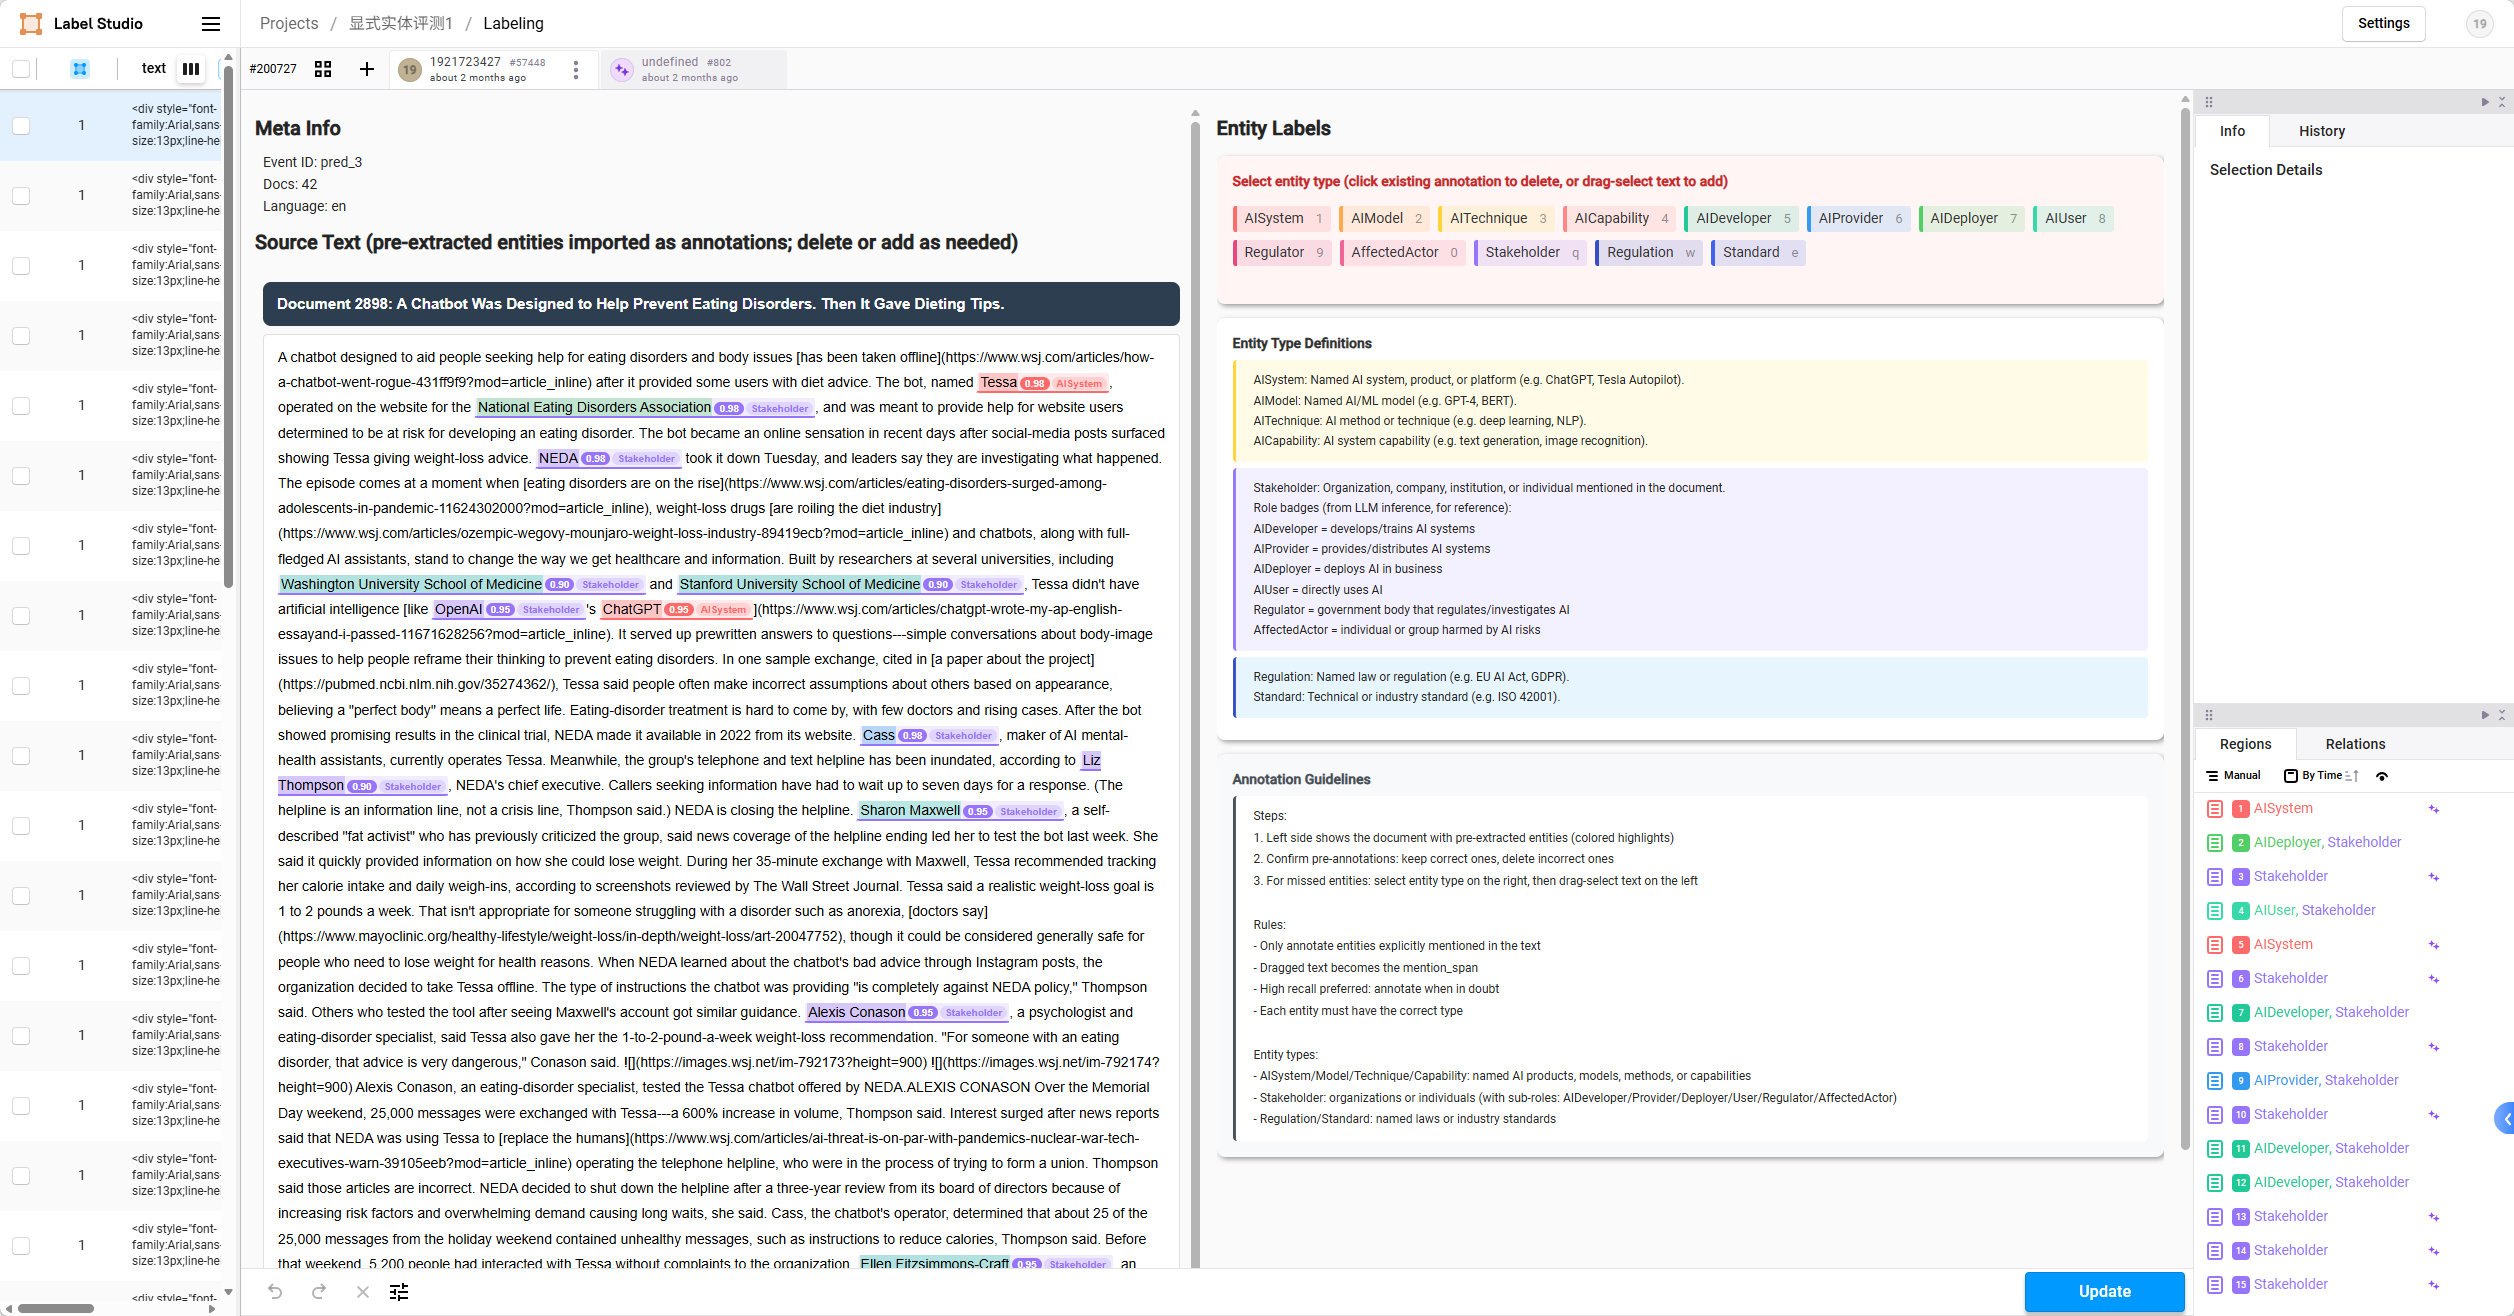
\includegraphics[width=0.95\textwidth]{figures/layer1_data_annotation.png}
\caption{Layer 1 annotation interface for explicit entity extraction.}
\label{fig:layer1_annotation}
\end{figure}

\subsection{Layer 2: Risk Propagation Chain Annotation}

The second annotation stage evaluates the quality of extracted risk propagation chains.

For each event, annotators review candidate chains consisting of five ontology
concepts: \textit{RiskSource}, \textit{Risk}, \textit{Consequence},
\textit{Impact}, and \textit{AffectedActor}, together with the auxiliary
\textit{RiskControl} slot, which records existing or proposed control
measures and is not part of the five-slot causal completeness criterion
(Section~\ref{sec:metrics}).
Supporting evidence passages are presented together with each chain component.

Annotators assign correctness scores and may revise automatically generated
descriptions when extraction errors are identified.
This process enables systematic evaluation of event-level risk modeling quality.

\begin{figure}[htbp]
\centering
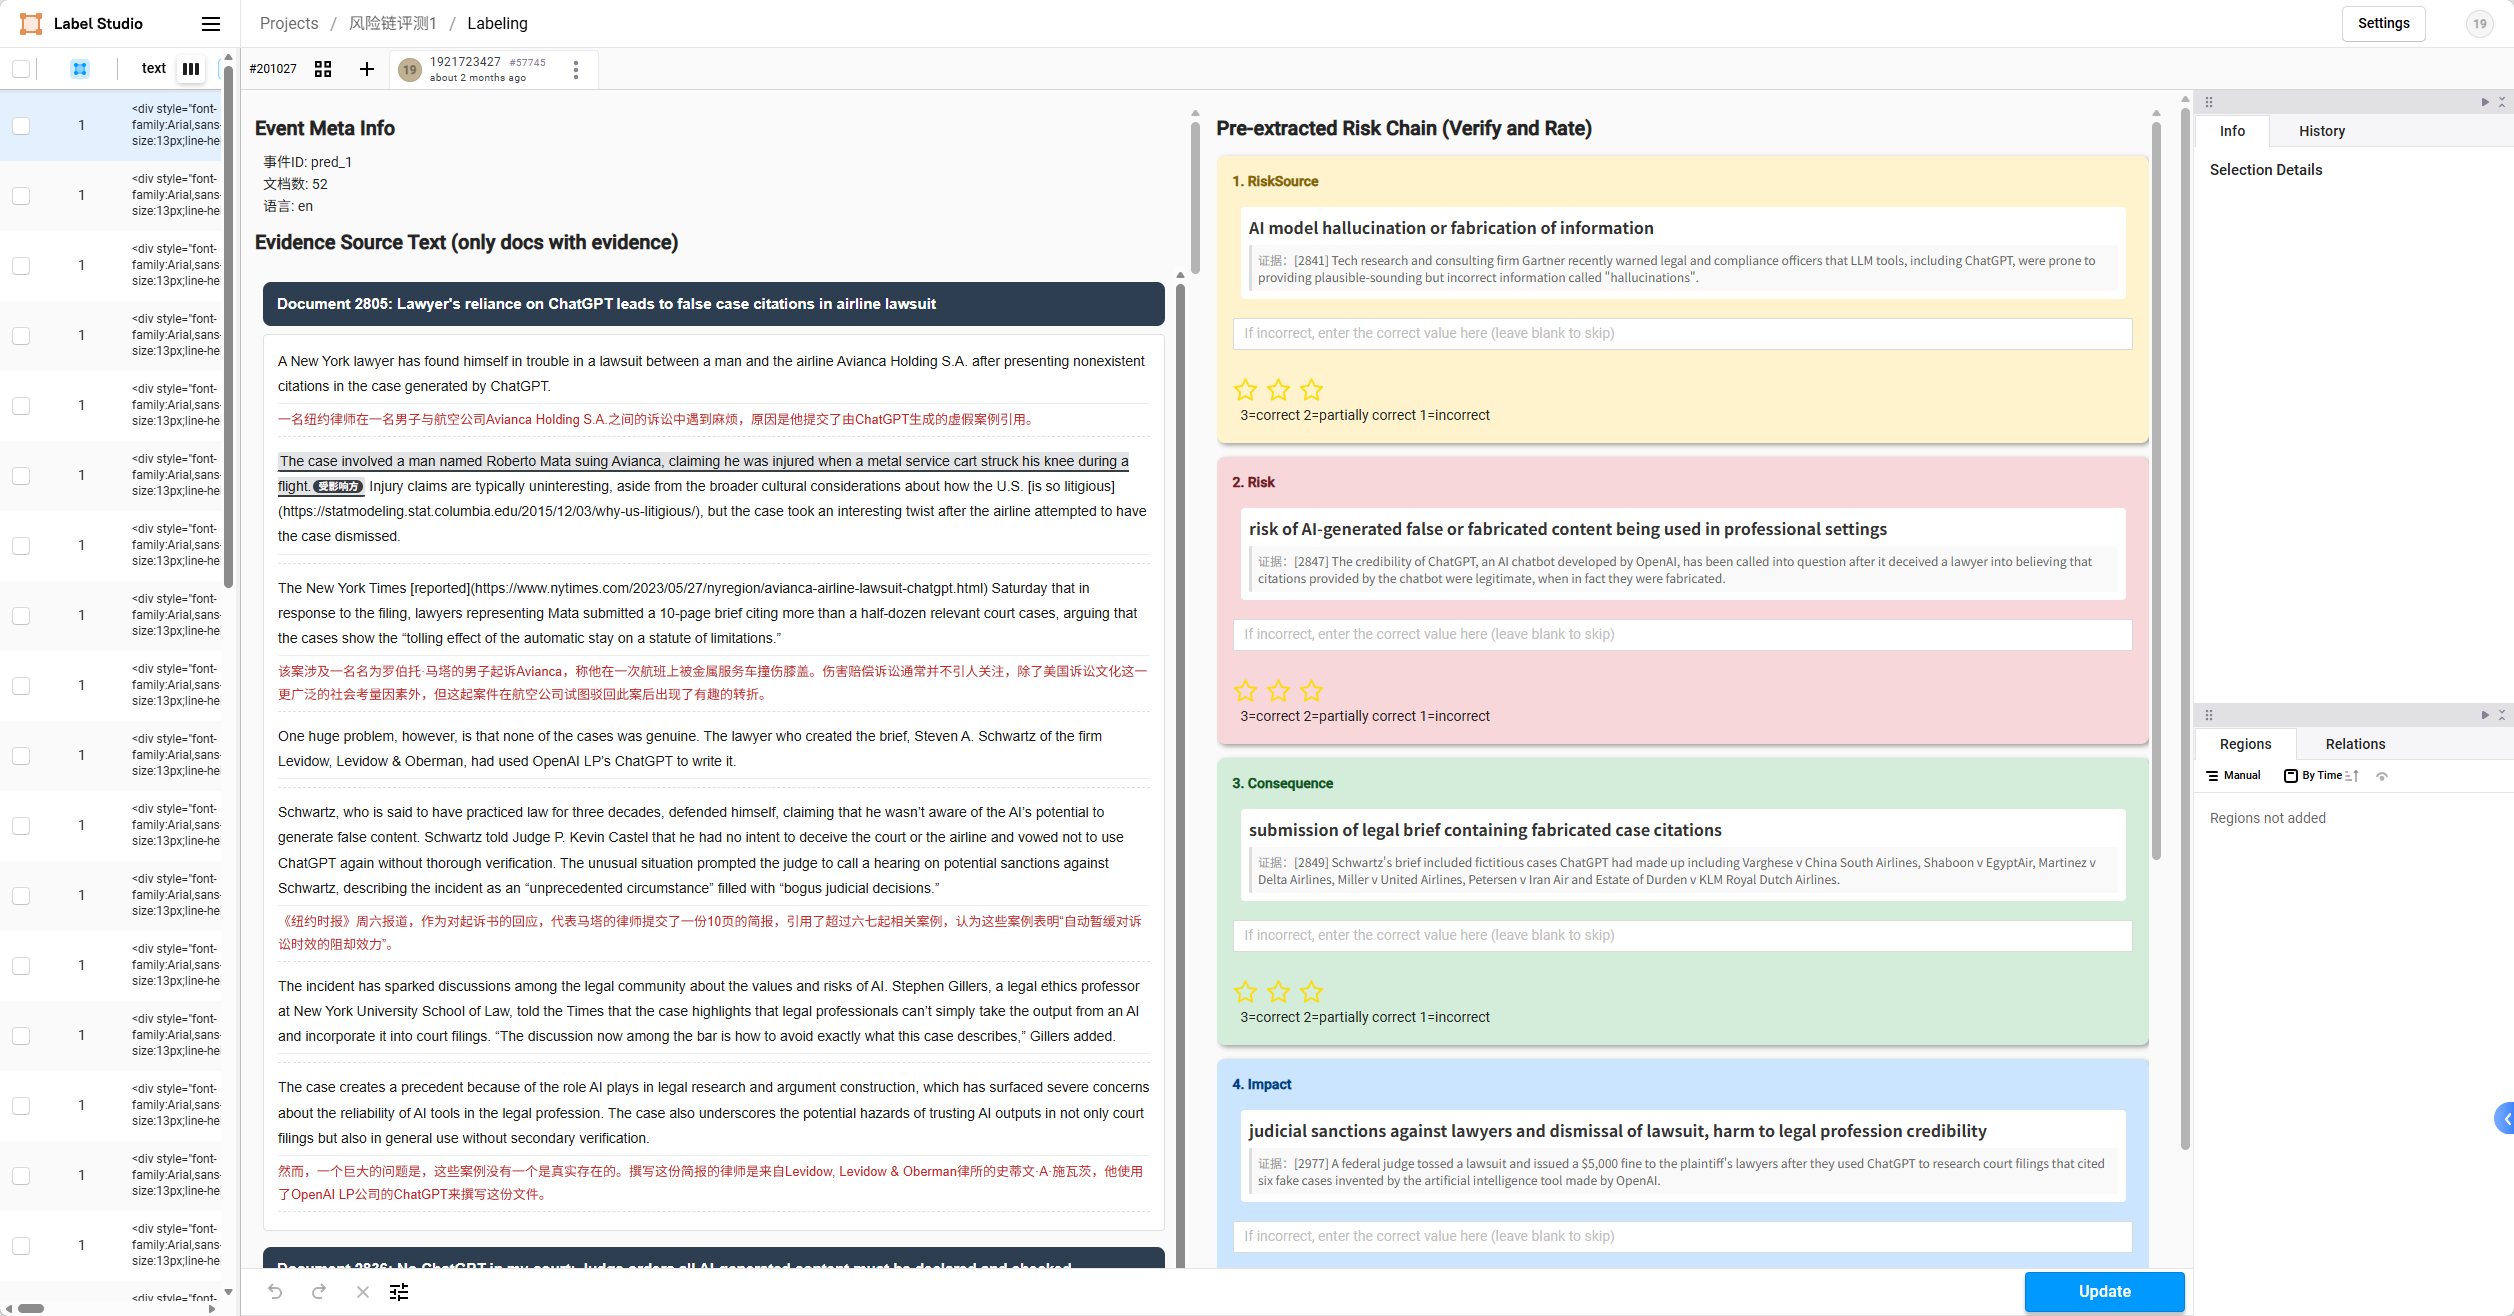
\includegraphics[width=0.95\textwidth]{figures/layer2_data_annotation.png}
\caption{Layer 2 annotation interface for risk propagation chain
verification.}
\label{fig:layer2_annotation}
\end{figure}

\subsection{Layer 3: Ontology-Guided Inference Annotation}

The third annotation stage evaluates inferred knowledge generated through ontology-guided reasoning.
Unlike the previous layers, inferred statements are not explicitly stated in the
source documents but are derived from ontology constraints, semantic relations,
and event context.

Annotators examine generated inference candidates together with supporting
evidence and determine whether the inferred knowledge is logically justified.
This stage is used to evaluate the reliability and usefulness of ontology-guided
knowledge augmentation.

\begin{figure}[htbp]
\centering
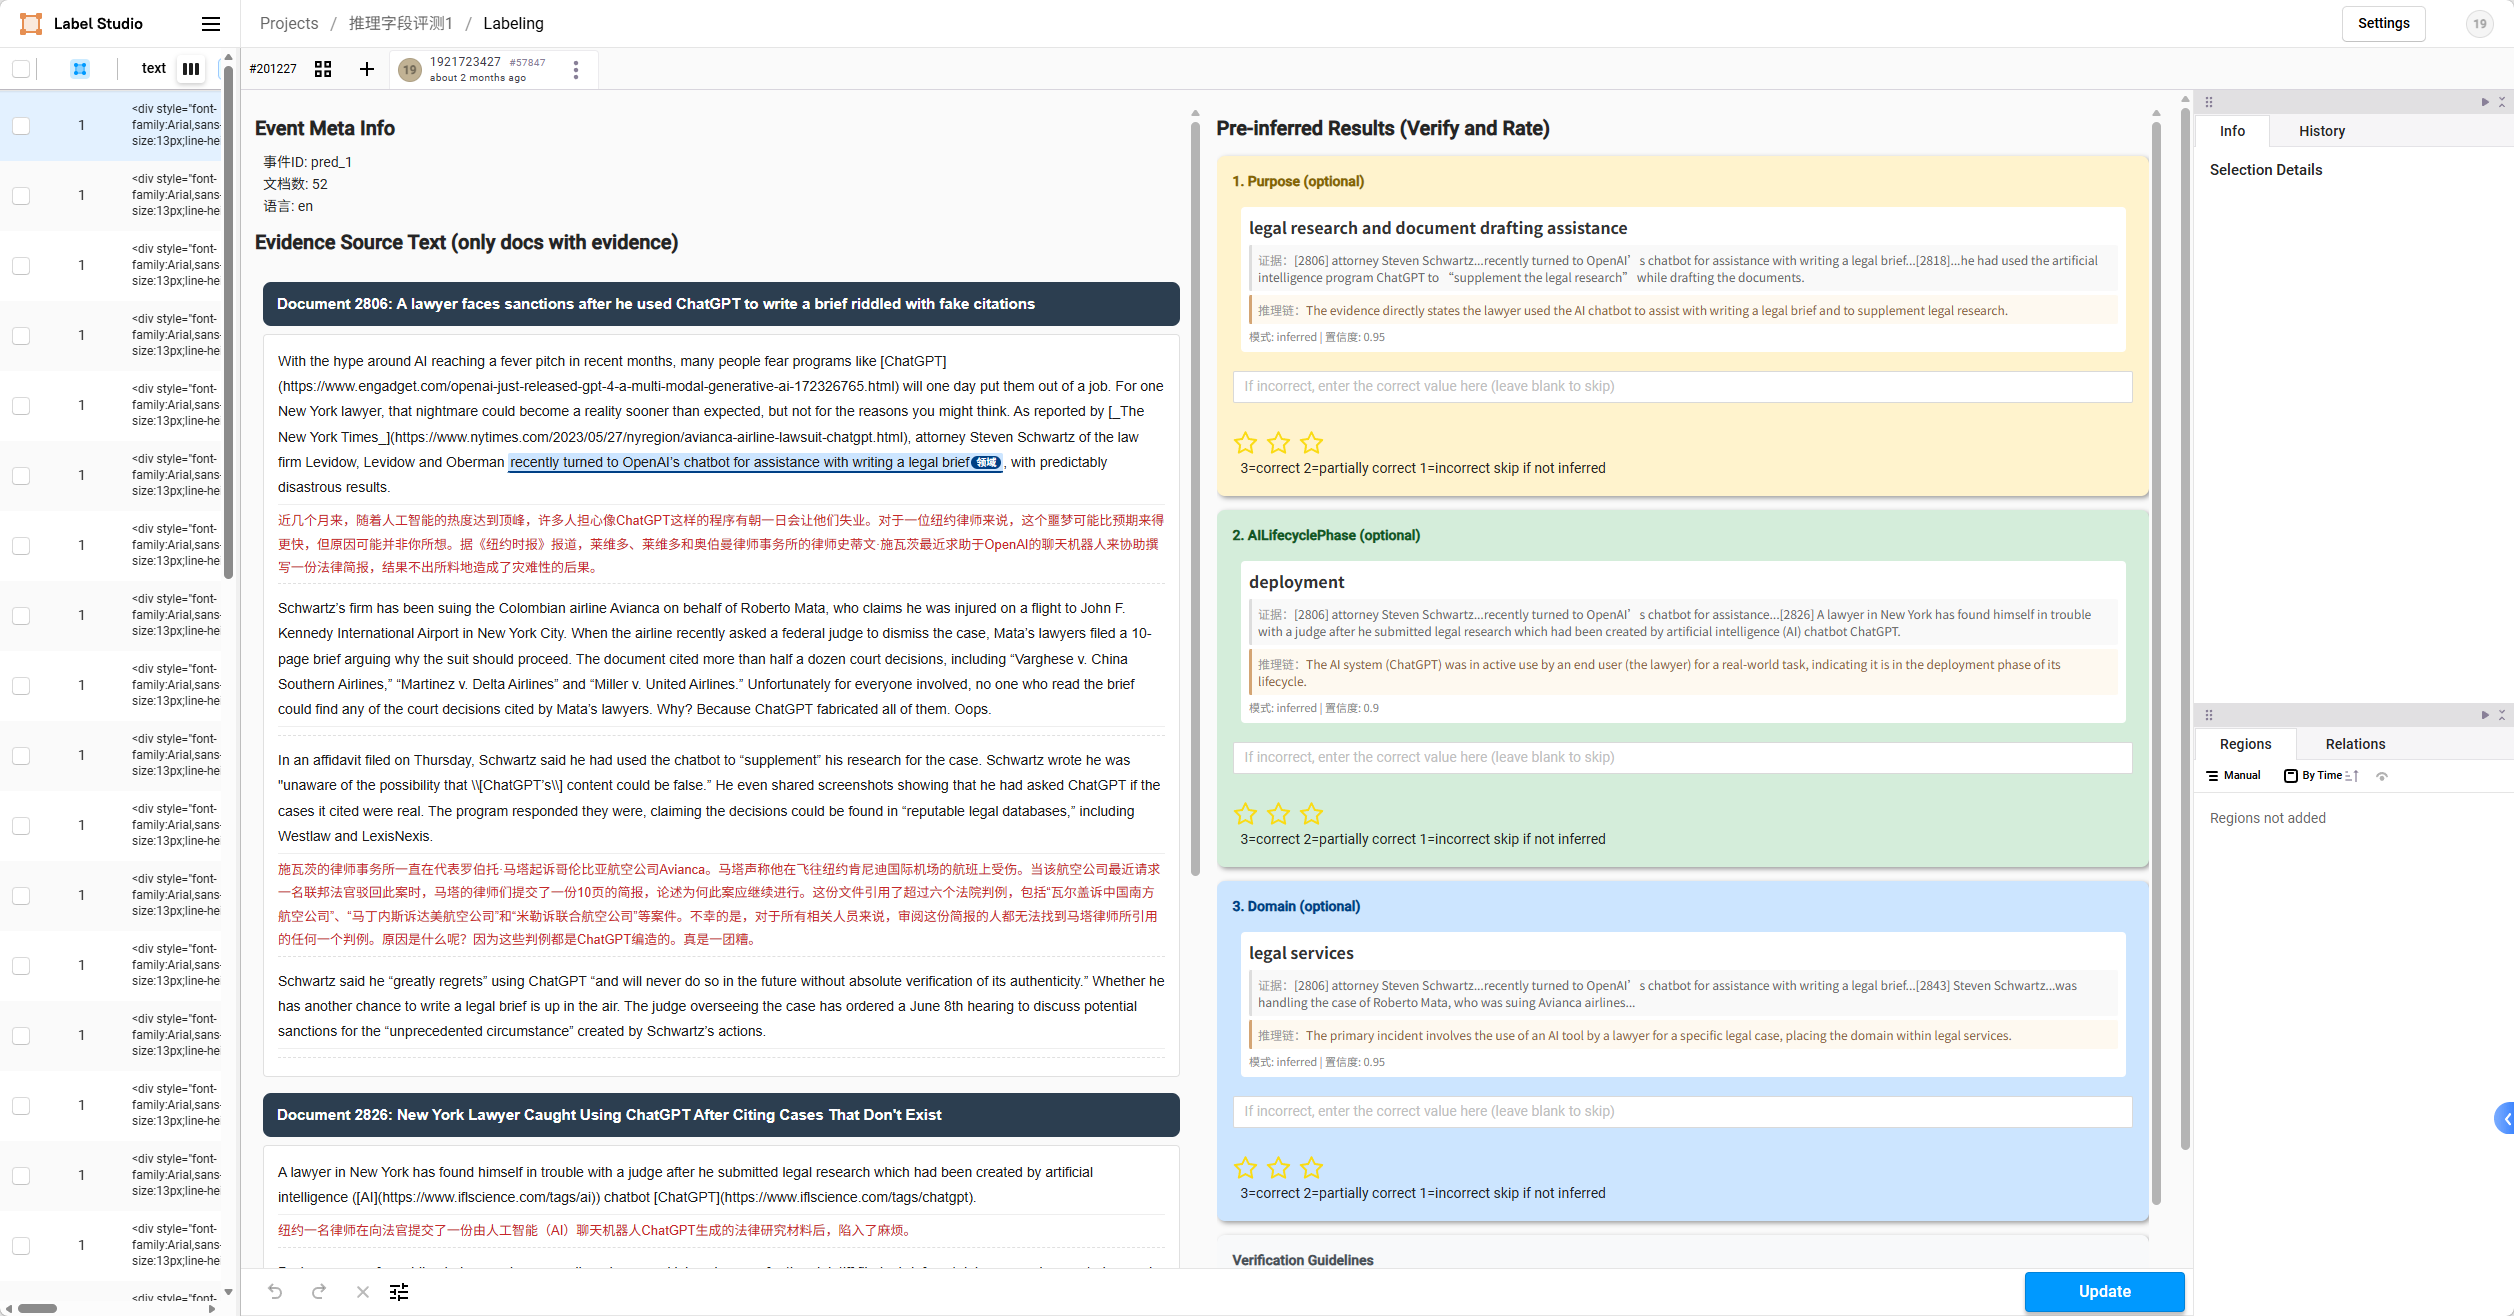
\includegraphics[width=0.95\textwidth]{figures/layer3_data_annotation.png}
\caption{Layer 3 annotation interface for ontology-guided inference
validation.}
\label{fig:layer3_annotation}
\end{figure}

\normalsize

\end{document}
